%  LaTeX support: latex@mdpi.com 
%  In case you need support, please attach all files that are necessary for compiling as well as the log file, and specify the details of your LaTeX setup (which operating system and LaTeX version / tools you are using).

%=================================================================
\documentclass[journal,article,submit,moreauthors,pdftex]{Definitions/mdpi} 

\usepackage{tabularx,colortbl}
\usepackage{booktabs} % For formal tables
\usepackage{array}
\usepackage{multirow}
\usepackage{subcaption}


\newcommand{\emad}[1]{\textcolor{red}{{\it [Emad: #1]}}}
\newcommand{\hosein}[1]{\textcolor{orange}{{\it [Hosein: #1]}}}
\newcommand{\diego}[1]{\textcolor{gray}{{\it [Diego: #1]}}}
\newcommand{\todo}[1]{\colorbox{yellow}{\textbf{[#1]}}}

% If you would like to post an early version of this manuscript as a preprint, you may use preprint as the journal and change 'submit' to 'accept'. The document class line would be, e.g., \documentclass[preprints,article,accept,moreauthors,pdftex]{mdpi}. This is especially recommended for submission to arXiv, where line numbers should be removed before posting. For preprints.org, the editorial staff will make this change immediately prior to posting.

%--------------------
% Class Options:
%--------------------
%----------
% journal
%----------
% Choose between the following MDPI journals:
% acoustics, actuators, addictions, admsci, aerospace, agriculture, agriengineering, agronomy, algorithms, animals, antibiotics, antibodies, antioxidants, applsci, arts, asc, asi, atmosphere, atoms, axioms, batteries, bdcc, behavsci , beverages, bioengineering, biology, biomedicines, biomimetics, biomolecules, biosensors, brainsci , buildings, cancers, carbon , catalysts, cells, ceramics, challenges, chemengineering, chemistry, chemosensors, children, cleantechnol, climate, clockssleep, cmd, coatings, colloids, computation, computers, condensedmatter, cosmetics, cryptography, crystals, dairy, data, dentistry, designs , diagnostics, diseases, diversity, drones, econometrics, economies, education, electrochem, electronics, energies, entropy, environments, epigenomes, est, fermentation, fibers, fire, fishes, fluids, foods, forecasting, forests, fractalfract, futureinternet, futurephys, galaxies, games, gastrointestdisord, gels, genealogy, genes, geohazards, geosciences, geriatrics, hazardousmatters, healthcare, heritage, highthroughput, horticulturae, humanities, hydrology, ijerph, ijfs, ijgi, ijms, ijtpp, informatics, information, infrastructures, inorganics, insects, instruments, inventions, iot, j, jcdd, jcm, jcp, jcs, jdb, jfb, jfmk, jimaging, jintelligence, jlpea, jmmp, jmse, jnt, jof, joitmc, jpm, jrfm, jsan, land, languages, laws, life, literature, logistics, lubricants, machines, magnetochemistry, make, marinedrugs, materials, mathematics, mca, medicina, medicines, medsci, membranes, metabolites, metals, microarrays, micromachines, microorganisms, minerals, modelling, molbank, molecules, mps, mti, nanomaterials, ncrna, neonatalscreening, neuroglia, nitrogen, notspecified, nutrients, ohbm, particles, pathogens, pharmaceuticals, pharmaceutics, pharmacy, philosophies, photonics, physics, plants, plasma, polymers, polysaccharides, preprints , proceedings, processes, proteomes, psych, publications, quantumrep, quaternary, qubs, reactions, recycling, religions, remotesensing, reports, resources, risks, robotics, safety, sci, scipharm, sensors, separations, sexes, signals, sinusitis, smartcities, sna, societies, socsci, soilsystems, sports, standards, stats, surfaces, surgeries, sustainability, symmetry, systems, technologies, test, toxics, toxins, tropicalmed, universe, urbansci, vaccines, vehicles, vetsci, vibration, viruses, vision, water, wem, wevj

%---------
% article
%---------
% The default type of manuscript is "article", but can be replaced by: 
% abstract, addendum, article, benchmark, book, bookreview, briefreport, casereport, changes, comment, commentary, communication, conceptpaper, conferenceproceedings, correction, conferencereport, expressionofconcern, extendedabstract, meetingreport, creative, datadescriptor, discussion, editorial, essay, erratum, hypothesis, interestingimages, letter, meetingreport, newbookreceived, obituary, opinion, projectreport, reply, retraction, review, perspective, protocol, shortnote, supfile, technicalnote, viewpoint
% supfile = supplementary materials

%----------
% submit
%----------
% The class option "submit" will be changed to "accept" by the Editorial Office when the paper is accepted. This will only make changes to the frontpage (e.g., the logo of the journal will get visible), the headings, and the copyright information. Also, line numbering will be removed. Journal info and pagination for accepted papers will also be assigned by the Editorial Office.

%------------------
% moreauthors
%------------------
% If there is only one author the class option oneauthor should be used. Otherwise use the class option moreauthors.

%---------
% pdftex
%---------
% The option pdftex is for use with pdfLaTeX. If eps figures are used, remove the option pdftex and use LaTeX and dvi2pdf.

%=================================================================
\firstpage{1} 
\makeatletter 
\setcounter{page}{\@firstpage} 
\makeatother
\pubvolume{xx}
\issuenum{1}
\articlenumber{5}
\pubyear{2019}
\copyrightyear{2019}
%\externaleditor{Academic Editor: name}
\history{Received: date; Accepted: date; Published: date}
%\updates{yes} % If there is an update available, un-comment this line

%% MDPI internal command: uncomment if new journal that already uses continuous page numbers 
%\continuouspages{yes}

%------------------------------------------------------------------
% The following line should be uncommented if the LaTeX file is uploaded to arXiv.org
%\pdfoutput=1

%=================================================================
% Add packages and commands here. The following packages are loaded in our class file: fontenc, calc, indentfirst, fancyhdr, graphicx, lastpage, ifthen, lineno, float, amsmath, setspace, enumitem, mathpazo, booktabs, titlesec, etoolbox, amsthm, hyphenat, natbib, hyperref, footmisc, geometry, caption, url, mdframed, tabto, soul, multirow, microtype, tikz

%=================================================================
%% Please use the following mathematics environments: Theorem, Lemma, Corollary, Proposition, Characterization, Property, Problem, Example, ExamplesandDefinitions, Hypothesis, Remark, Definition
%% For proofs, please use the proof environment (the amsthm package is loaded by the MDPI class).

%=================================================================
% Full title of the paper (Capitalized)
\Title{Comparative Study on Hand-Crafted Features for Human Activity Recognition Using Sensory Data}

% Author Orchid ID: enter ID or remove command
\newcommand{\orcidauthorA}{0000-0000-000-000X} % Add \orcidA{} behind the author's name
%\newcommand{\orcidauthorB}{0000-0000-000-000X} % Add \orcidB{} behind the author's name

% Authors, for the paper (add full first names)
\Author{Hosein Nourani $^{1,\dagger,\ddagger}$\orcidA{} and Emad Shihab $^{1,\ddagger}$ }

% Authors, for metadata in PDF
\AuthorNames{Hosein Nourani and Emad Shihab}

% Affiliations / Addresses (Add [1] after \address if there is only one affiliation.)
\address{%
$^{1}$ \quad Dept. of Computer Science and Software Engineering; h$.$nourani@hotmail.com\\
$^{2}$ \quad Dept. of Computer Science and Software Engineering; e$.$shihab@concordia.com}

% Contact information of the corresponding author
\corres{Correspondence: e-mail@e-mail.com; Tel.: (optional; include country code; if there are multiple corresponding authors, add author initials) +xx-xxxx-xxx-xxxx (F.L.)}

% Current address and/or shared authorship
\firstnote{Current address: Affiliation 3} 
\secondnote{These authors contributed equally to this work.}
% The commands \thirdnote{} till \eighthnote{} are available for further notes

%\simplesumm{} % Simple summary

%\conference{} % An extended version of a conference paper

% Abstract (Do not insert blank lines, i.e. \\) 
\abstract{Human Activity Recognition (HAR) using sensory data refers to an emerging area of interest for healthcare, military, and security applications. Several researches are conducted to capture a certain activity from an stream of data. Basically, the most popular methods extract some attributes (features) of a signal and apply a pattern recognition model on them. There are several studies that they have proposed different set of features that show the performance is significantly improved. However, since each result have been achieved under its own setup, comparing the impact of different featuresets can not be made in a distinct form. Therefore, in this work, we split a HAR setup into its three main characteristics including dataset (types of activities), classifiers, and evaluation methods; Then, we assess the impact of using different featuresets in each characteristic of setup, separately. Toward this end, we address three challenges: (1) choosing featureset, (2) choosing classifier, and (3) choosing evaluation method. We present cross-validation results on 20 different models using 5 featuresets and 4 classifiers. For experiments, We create a dataset of 8 complex gym exercises from 13 subjects over several sessions. Results showed that models on histogram-bin features deliver the best performance (on average 87.80\% of F1) relatively better than general statistical features. Among classifiers, the average classification performance of Forward Neural Network (FNN) model is reported the highest performance (95.89\% of F1) using histogram bins in k-fold cross-validation. FNN in Leave-One-Trial-Out cross-validation and Leave-One-Subject-Out cross-validation achieved 89.66\% and 81.59\% respectively. This study provides significant experimental results on building a HAR model under realistic conditions.
}
% Keywords
\keyword{Feature Extraction; Featureset; Wearable; Motion Sensor; Neural Network, Histogram, Human Activity Recognition }

% The fields PACS, MSC, and JEL may be left empty or commented out if not applicable
%\PACS{J0101}
%\MSC{}
%\JEL{}

%%%%%%%%%%%%%%%%%%%%%%%%%%%%%%%%%%%%%%%%%%
% Only for the journal Diversity
%\LSID{\url{http://}}

%%%%%%%%%%%%%%%%%%%%%%%%%%%%%%%%%%%%%%%%%%
% Only for the journal Applied Sciences:
%\featuredapplication{Authors are encouraged to provide a concise description of the specific application or a potential application of the work. This section is not mandatory.}
%%%%%%%%%%%%%%%%%%%%%%%%%%%%%%%%%%%%%%%%%%

%%%%%%%%%%%%%%%%%%%%%%%%%%%%%%%%%%%%%%%%%%
% Only for the journal Data:
%\dataset{DOI number or link to the deposited data set in cases where the data set is published or set to be published separately. If the data set is submitted and will be published as a supplement to this paper in the journal Data, this field will be filled by the editors of the journal. In this case, please make sure to submit the data set as a supplement when entering your manuscript into our manuscript editorial system.}

%\datasetlicense{license under which the data set is made available (CC0, CC-BY, CC-BY-SA, CC-BY-NC, etc.)}

%%%%%%%%%%%%%%%%%%%%%%%%%%%%%%%%%%%%%%%%%%
% Only for the journal Toxins
%\keycontribution{The breakthroughs or highlights of the manuscript. Authors can write one or two sentences to describe the most important part of the paper.}

%\setcounter{secnumdepth}{4}
%%%%%%%%%%%%%%%%%%%%%%%%%%%%%%%%%%%%%%%%%%
\begin{document}
%%%%%%%%%%%%%%%%%%%%%%%%%%%%%%%%%%%%%%%%%%

%%%%%%%%%%%%%%%%%%%%%%%%%%%%%%%%%%%%%%%%%%
%The order of the section titles is: Introduction, Materials and Methods, Results, Discussion, Conclusions for these journals: aerospace,algorithms,antibodies,antioxidants,atmosphere,axioms,biomedicines,carbon,crystals,designs,diagnostics,environments,fermentation,fluids,forests,fractalfract,informatics,information,inventions,jfmk,jrfm,lubricants,neonatalscreening,neuroglia,particles,pharmaceutics,polymers,processes,technologies,viruses,vision

\section{Introduction}

%The introduction should briefly place the study in a broad context and highlight why it is important. It should define the purpose of the work and its significance. The current state of the research field should be reviewed carefully and key publications cited. Please highlight controversial and diverging hypotheses when necessary. Finally, briefly mention the main aim of the work and highlight the principal conclusions. As far as possible, please keep the introduction comprehensible to scientists outside your particular field of research. Citing a journal paper \cite{ref-journal}. And now citing a book reference \cite{ref-book}. Please use the command \citep{ref-journal} for the following MDPI journals, which use author-date citation: Administrative Sciences, Arts, Econometrics, Economies, Genealogy, Humanities, IJFS, JRFM, Languages, Laws, Religions, Risks, Social Sciences.
%%%%%%%%%%%%%%%%%%%%%%%%%%%%%%%%%%%%%%%%%%
With the rise of life expectancy and ageing of the population, the development of new technologies that focus on elderly healthcare has become a challenge \cite{hong2008activity}.
Human Activity Recognition (HAR) using on-body sensing is one of the most prevalent assistive technologies to support older people's daily life ~\cite{wang2019survey}. As such, in about a decade, extensive researches have been undertaken in this regard and, in result, several outstanding high-performance HAR models have been proposed with an accuracy almost 100\% in several scopes - fall risk assessment \cite{sow2013mining}, physical fitness monitoring\cite{morris2014recofit}, or medical diagnosis \cite{gonzalez2015features}, to name but a few, which made HAR a very promising realm, consequently. In addition, using Wearables (i.e., smartphones, smartwatches) is increasingly pervasive. Wearables are small in size, relatively cheap and ubiquitously used, reveal numerous new potentials for HAR systems in research and industry. However, by no means should we lose sight of the fact that these advances in wearable devices require a constant upgrading on models' environments which is essential to utilize the maximum capabilities of the device, resulting an overall performance improvement. In practice, employing a high-performance HAR model in an upgraded setup does not grant a better accuracy or even as equal as it used to be in the initial setup. This is mainly because the HAR models are mostly designed under particular environment setup which is hindering the adaptability to the new environment which called \textit{lack of generalizability} - one well-known reason mentioned in several previous studies \cite{schilit1994context, soro2019recognition, shoaib2016complex}. Since a HAR approach composed of independent phases where each phase plays a crucial role in acquiring the ultimate performance, a distinction on generalizability of each phase is very essential to address the issue. Nevertheless, to the best of our knowledge, only a few studies conducted a phase-by-phase investigation on HAR models. Therefore, the purpose of this study is a phase comparison of the state-of-the-art HAR systems, aiming to highlight the generalizable parts of each approach.\\

\subsection{Human Activity Recognition Approach}
% explain the approach + highlighting the feature extraction as the most important phase
Wearable sensor-based HAR systems basically share a similar approach ~\cite{s140610146}. This approach is shown in Figure \ref{fig:main_approach}. The procedure starts with capturing an activity into time series signal using inertial on-body sensors (i.e., accelerometer, gyroscope) and storing it into a dataset. Next, the stream splits into segments while each segment is labelled with the activity performed within that segment. To be used in classification model, each segment of data is summarized into a feature vector, during the feature extraction phase. Extracting a feature vector from a segment of data plays a crucial step in HAR process. engineering a limited set of features, efficiently provide the most relevant characteristics of data for the classifier is still subject to research. 

\begin{figure}[H]
	\centering
	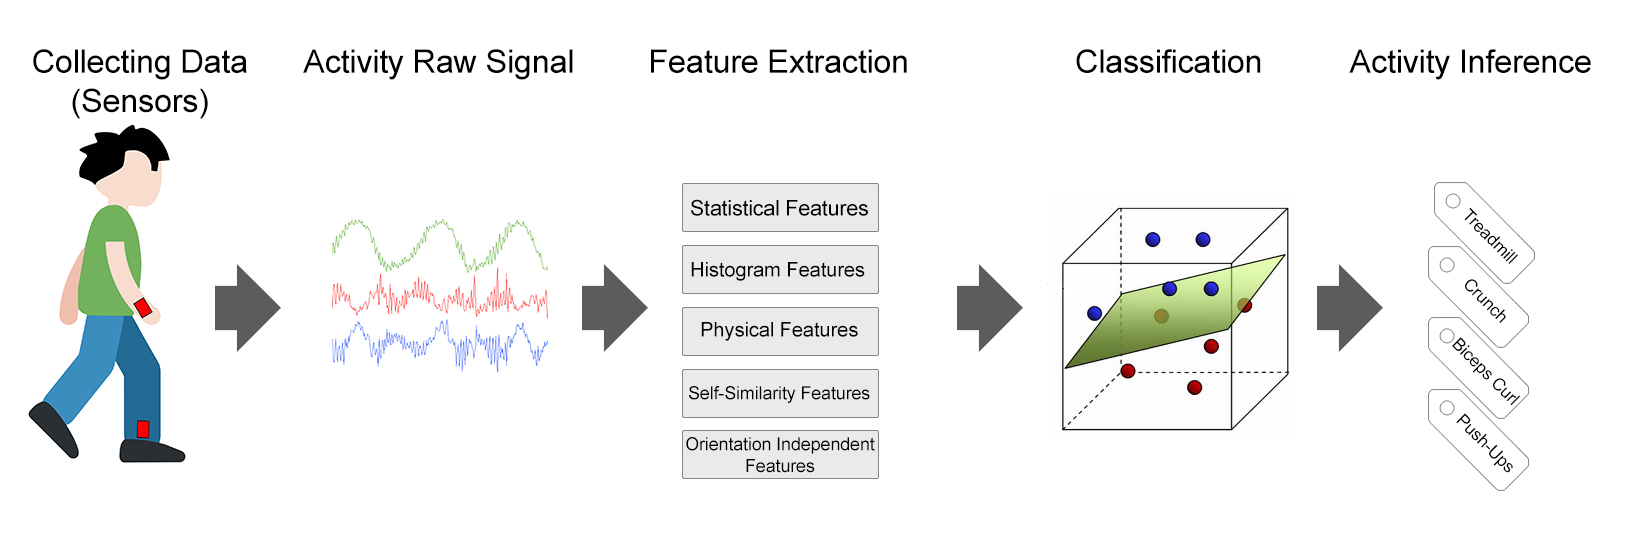
\includegraphics[width=15.5 cm]{Definitions/images/main_approach.jpg}
	\caption{Typical Work-flow on Human Activity Recognition}
	\label{fig:main_approach}
\end{figure} 

\subsection{Feature Engineering in HAR}
Providing an efficient set of feature for a recognition model has two main steps: 1) feature extraction 2) feature selection. Particularly in HAR, extracting features is based on a comprehensive understanding of the activity's movements in a coordinate system~\cite{}; While, selecting features is a heuristic filtering approach on features to minimize their redundancy and maximize their relevancy to the activity~\cite{}. Theoretically, any distinctive characteristic of an activity is an intuition to be developed as a feature.
Although feature selection is not a mandatory step in HAR pipeline, employing feature selection is very popular as it proved that it can significantly improves the performance. There are several studies have shown that the featureset returned from the feature selection improves the model's performance both in accuracy and computational costs~\cite{rosati2018comparison, Nourani_CoMoRea2019, wang2019survey}. For example, in our previous study, we setup an study/experiment on time domain features and used an ensemble feature selection and showed that using only 10\% of features the performance is still identical.or ~\cite{yazdansepas2016multi}. Mohamd shoeib extract x number of features and manually split them into four sets of features and trained one model per each. the performance difference between models was up to 30\% (65\% for time domain features to 95\% for combination of time and frequency domain features).\\
Therefore, the performance achieved by a featureset depends on both steps which are tightly bound up with each other. 


%grouping the featuresets based on the undestanding of the activities



The data collected by sensors as \textit{time series raw signal} will be segmented into smaller pieces (Figure \ref{fig:main_approach} step 2) to become easier on classification phase. In step 3, useful representative features (e.g., statistical features) for distinguishing activities are extracted from each segment - \textit{feature extraction}\cite{rosati2018comparison, wang2019survey}. The data extracted from step 3 will be considered as input for \textit{classification} in step 4. The classification output is the activity name in step 5. At this step, different \textit{evaluation} method can asses the performance of the model.\\


Basically, extracting features is based on a comprehensive understanding of physically how an activity has been done. Among different type of features, statistical features has been received the most attention in HAR studies. However, in recent years, other type of features, like frequency domain features and hybrid features have been combined with statistical features with the aim of improving activity recognition performance\cite{wang2019survey, morris2014recofit}. Although there are several studies in literature that show these featuresets outcome remarkable model performance, to the best of our knowledge, there is no empirical study investigating the performance of each set of features. Specifically, there is not a comparison study, considering different classifiers and evaluation methods under same dataset and experimental setup. One simple solution is to extract more features, however, more number of features causes more energy consumption, which can be problematic for an energy-limited device, like a smartphone\cite{Nourani_CoMoRea2019}. Hence, such a detailed analysis can help in deciding when to best use each set of features. Therefore, there is a need to study the impact of these featureset in detail. In particular, we focus on this research question: "How and when are various featuresets, which are all state-of-the-art, best used for better recognition performance (RQ1)".

Some researchers have already investigated the impact of various features in activity recognition\cite{morris2014recofit,zhang2013human, rosati2018comparison}. For example, in \cite{morris2014recofit}, the authors use statistical features in combination with auto-correlation features using SVM classifier and report a robust HAR system on gym exercises with around 99\% of accuracy on their own dataset. On the other hand, in \cite{zhang2011feature}, the authors claim that the addition of physical features, feature based on physical interpretation, to statistical features while employing a multi-level classification, improves the performance to 90\% of accuracy. Although the first study has reached a better performance than second study, it does not necessarily mean that the auto-correlation features are 9\% more informative than physical features. These two papers are showing different results probably due to their different experimental setups. In order to compare the impact of each featureset, it is important to examine them under same experimental setup. However, these previous studies have investigated featuresets on different dataset and classification method. In order to have general answer to RQ1, we need to know the role of other factors like classification method on HAR model. In other words, we are aiming to answer: "How different do classifiers perform on different featuresets (RQ2)". We chose four classifiers in order to cover the most commonly used classification methods in the previous studies. These classifiers are: Support-Vector Machine (SVM), Feed-Forward Network (FNN), Decision Tree (DT), and K-Nearest Neighbor (KNN).

In 2018, Jordao et al. \cite{jordao2018human} revealed a basic issue regarding the process of extracting features. They showed that the traditional process of generating data points is vulnerable to bias leading skewed results. It occurs because the part of the sample's content can appear in training and testing, simultaneously. They have demonstrated that by applying non-biased ways of generating features from raw data, recognition performance has been significantly affected. Therefore, in this study we also investigate impact of three protocol of generating features: A: Extracting features over whole dataset (traditional method), B: Extracting features over sessions of recording data, and C: Extracting features over data of each subject separated. Method A is selected because it was mostly-used in previous studies \cite{}. There is an evaluation method corresponding with each way of generating features including K-fold, Leave-One-Trial-Out (LOTO), and Leave-One-Subject-Out (LOSO), respectively. In particular, we want to answer this research question: "How do different protocols impact on recognition performance? (RQ3)".\\

We believe that our effort will assist the readership and this will save time for future studies by not repeating the same experiments. This study can be used as a basis for making design decisions about when and what to choose these set of features for better activity recognition. The main contributions and highlights of this paper are as follows:


\begin{itemize}
	\item To the best of our knowledge, we are the first to do such an extensive analysis of the role of state-of-the-art featuresets in activity recognition, over different classifiers and evaluation methods. We extract features from two sensors equipped with accelerometer and gyroscope on two body positions (wrist and foot). We have used four classification models in our experiments, which are all used in the state-of-the-art. 
	\item We also investigate the recognition performance when the features are orientation-independent comparing with when they are orientation-dependent. Moreover, we target a wide range of features from low complexity which are suitable for running on smartphones (e.g., histogram) to high complexity which are useful for online HAR systems\cite{morris2014recofit} for our evaluation scenarios.
	\item We introduce leave-one-set-out cross-validation which is similar to LOTO cross-validation. In addition, we show how much robust each state-of-the-art featureset is against different evaluation methods.
	\item We recognize eight gym exercises, commonly used in the state-of-the-art. Moreover, we make our data set and our labeling and extracting features application publicly available for future research in this domain \cite{gymDataset}.
\end{itemize}


The rest of the paper is organized as follows. We describe related work in Section 2. The data and the study setup including the approach and the dataset are explained in Section 3. The featuresets are described in Section 4 and our evaluation approach in Section 5. We discuss the performance evaluation in Section 6. Finally, we describe our conclusions and future work in Section 7.

--------------


Basically, a HAR system using Inertial Measurement Units (IMUs) is composed of two basic components: (1) a data acquisition unit responsible for capturing human movements, (2) a processing unit responsible for recognizing the certain activities among movements of the subject~\cite{rosati2018comparison}. In the first component, the human movements is captured by different motion sensors such as accelerometer, gyroscope, and so on. These sensors can be located in an off-the-shelf device like a smart-phone for general HAR applications or specifically are accompanied by a storage and a processor, formed a System on Chip (SoC) for a certain purpose. The captured movements as raw data transmits to the second component for processing operation.\\
Within the processing unit, there is a pattern recognition (HAR) model that classifies the input signals into certain classes of activities. This HAR model typically consists of three phases. First, there is a pre-processing operation that extracts informative features from raw signal. Second, a classifier is trained over extracted features. Third, an evaluation method to ensure that the classifier provides the required performance~\cite{kolodziej2019registration}. In other words, a HAR model should address these three aspects to be able to recognize an activity.

\section{Background}
The data coming from sensor depends on the type of sensor and the position of the sensor on the body.
accelerometer[] and gyroscope[] are the most popular sensor mostly used in HAR systems. the signal from magnetometer is sensitive against iron and local magnetic fields exist in the environment. therefore, it is less used rather the other sensors. to place the sensor on subject's body, previous works used different positions. authors have used chest, wrist, pocket, and foot to attach the sensor~\cite{hassan2018robust, morris2014recofit, s140610146, wang2019survey}. In this work, we used accelerometer and gyroscope located on two spots on wrist and on ankle.

\section{Related Work}

\subsection{Hand-crafted Features}

A large amount of researches have been conducted regarding the acquiring hand-crafted feature in preprocessing phase for recognizing human activities. In actual use, there are plenty of resources for a HAR model to receive the input. The hand-crafted features, manual functions to transform raw inputs into a more useful form for prediction, have proven to be effective and are gaining popularity\cite{wang2019survey}. This achieved due to the fact that, knowing a prior knowledge about the temporal pattern of a physical activity, researchers are able to extract those attributes of the signal that have correlation with that activity. For example, as can be seen in Figure \ref{fig:feature_intuition}, since the activity composed of two phases which in the second phase the wrist hits the highest point in x axis (the red circles in Figure \ref{fig:feature_intuition} (b)), the maximum value of x in each segment of signal can be used as a feature for a model to recognize "Dumbbell Triceps Dips". It is noteworthy that in this activity the wrist does not move significantly toward z axis, therefore, as it is shown in Figure \ref{fig:feature_intuition} (b), there is no significant information in the z signal to be extracted. In the section \ref{sec:feature_extraction}, there is a comprehensive explanation about different features and their intuitions.

\begin{figure}[H]
	\centering
	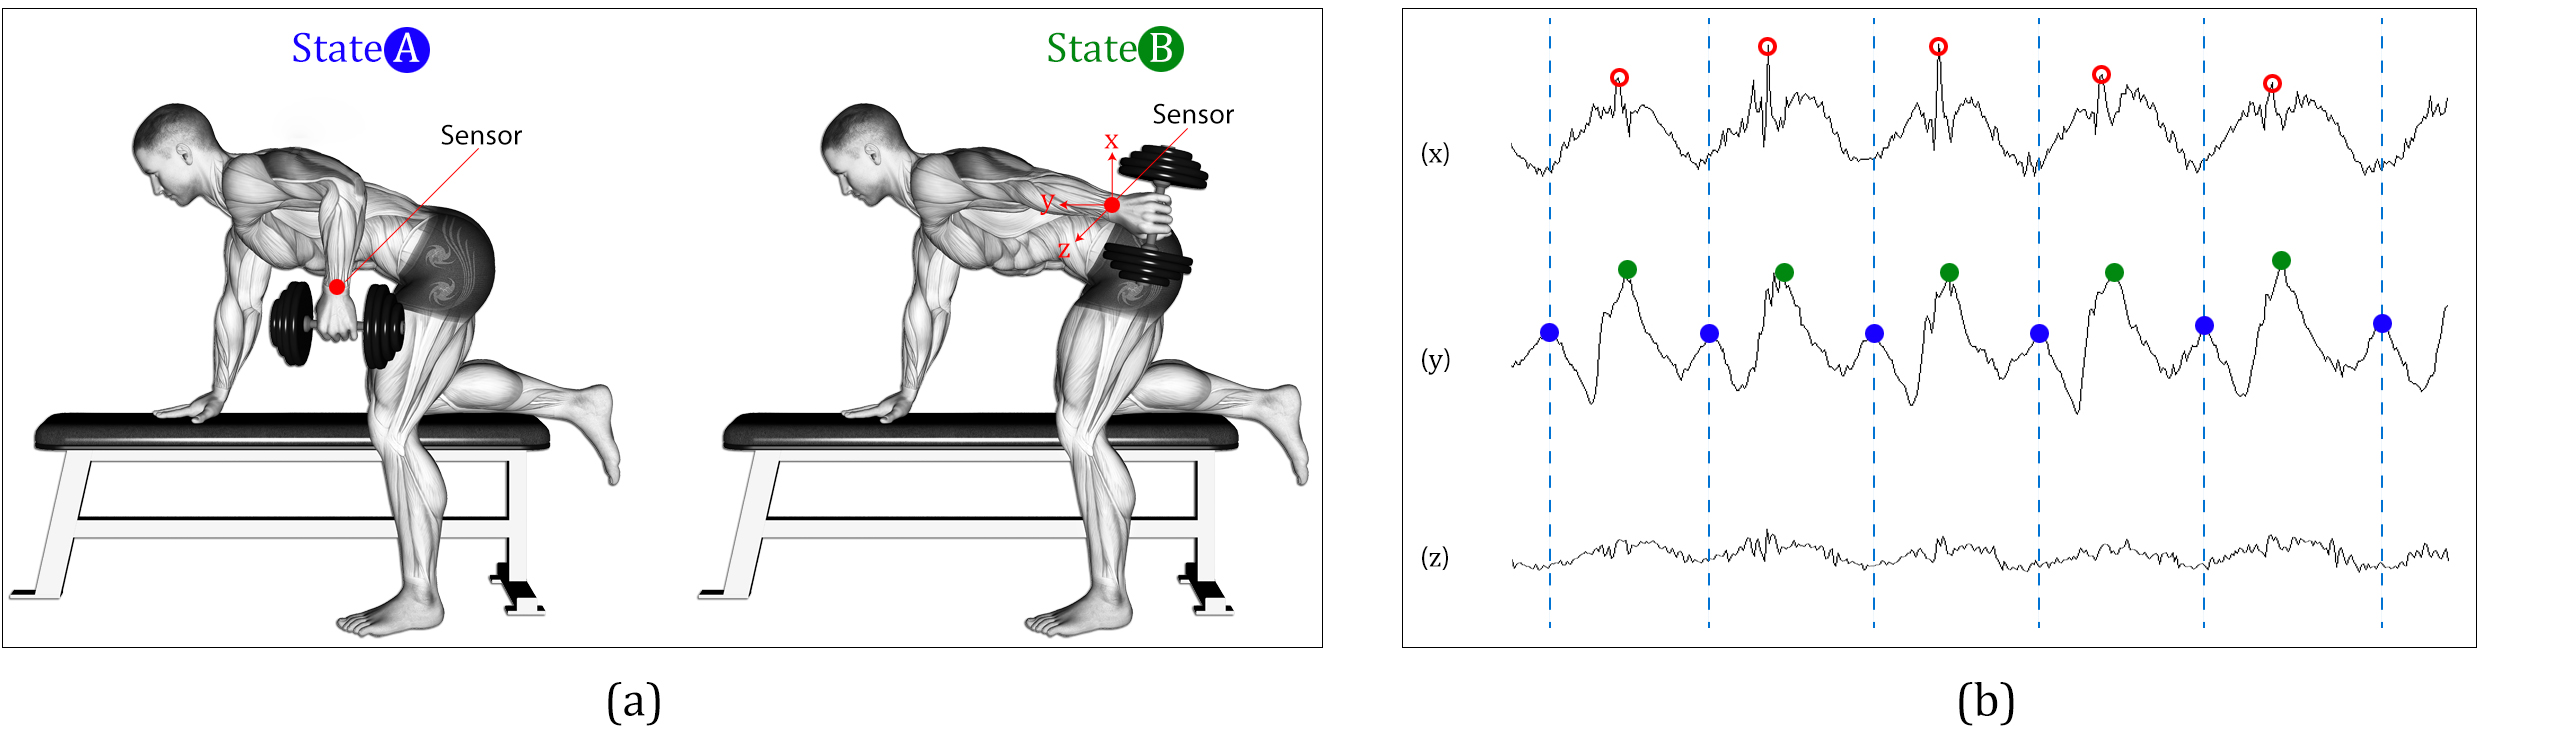
\includegraphics[width=14 cm]{Definitions/images/hand_craft_intuition.jpg}
	\caption{(a) Two states of "dumbbell triceps dips" while a sensor attached to the wrist. (b) The signals recorded by a triaxial accelerometer during five iteration of dumbbell triceps dips. Red and green bullets stand for State A and B respectively. The red circles indicate the maximum peaks in x signal. In feature extraction process, an input like the y axis signal might be considered as an intuitive feature such as mean or median to recognize each state of this activity.}
	\label{fig:feature_intuition}
\end{figure} 



Particularly, researchers have constructed various activity recognition models utilized the hand-crafted features. To this end the analysis of the activity per se is necessary. Wang et al. in \cite{wang2019survey} categorized human activities based on velocity and complexity (number of phases of doing the activity) into three main categories:
\begin{itemize}
	\item \textit{Basic activities}, repetitive activities during comparatively longer period e.g., walking and running. 
	\item \textit{Complex activities}, a sequence of several phases that each phase might be a complex or basic activity e.g., coffee time, smoking. 
	\item \textit{Transition activities} which having a certain behavior occurring between two different postures or two basic activities (e.g., stand-to-sit, push-ups).
\end{itemize}

From this point of view, introduced features in previous works mostly focused on a certain group of activities rather multiple categories altogether. For instance, Shoaib and Bosch setup an experiment with ten subjects to recognize seven \textit{basic activities} including running, sitting, standing, jogging, biking, walking upstairs and walking downstairs \cite{s140610146}. They extracted six time-domain features (Mean, standard deviation, median, zero crossings, root means square and variance) and two frequency domain features including sum of first five Fast-Fourier Transformation (FFT) coefficients and the spectral energy on the data of a triaxial accelerometer and a gyroscope. They achieved 96\% of accuracy using time-domain features while maximum 89\% when used frequency-domain features. Khokhlov et al. in \cite{khokhlov2018design} also targeted the basic activities in an experiment with seven subjects equipped by accelerometer and gyroscope on their showed that the combination of frequency-domain features and time-domain features improves the performance 
some studies focused on transition activities like x y z. there are also studies about complex activities like x and y, however they used other sensor modality like RFID in [] or oxygen intake sensor [] in their recognition. in this work, similar to \cite{morris2014recofit, }, , we focus on gym exercises a combination of basic and transition activities 





Some researchers have evaluated the effect of amending HAR performance with combining different set of features  ~\cite{yazdansepas2016multi, chen2018distilling}.


    Krishnan and Juillard setup a study \cite{krishnan2009recognition}

In [], authors developed a position-aware HAR system by placing seven accelerometers in different body positions.




Studies where a type of features was either used alone or in combination with another exist for many applications related to HAR.

For example, for gait analysis ~\cite{zhang2011feature, sprager2015inertial}, gym exercises ~\cite{rosati2018comparison} and disease diagnosis ~\cite{janidarmian2014automated}, the time domain features have been used, either alone or in combination with frequency domain features. Moreover, time domain features, frequency domain features, and a set of auto-correlation features combined to detect certain exercises in the gym \cite{morris2014recofit, rosati2018comparison}. \\
 

Rather than using a combination of features in a HAR model, There are studies in exploring and introducing new sets of hand-crafted features in the literature....

\subsection{Feature Selection}
In terms of accuracy and energy consumption, the number of used features matters. There are plenty of studies that aim to optimize the selection of features in a data driven way. In the process of selecting features, a subsection of the best individual features may not be a best set of features because of the possibility of redundancy among features which not only does not improve performance, but also increase the processing cost. Therefore, in practice, it may deteriorate the efficiency of the model[].% examples of feature selection methods
\subsection{HAR Evaluation}
To compare the performance of HAR models, in the literature, K-folds validation and cross-subject validation are more popular than others. [] uses 

\subsection{Featureset comparison}

While the extracting and applying hand-crafted features on HAR has been extensively studied ~\cite{wang2019survey,janidarmian2017comprehensive}, They less have done an empirical study that demonstrates a side-by-side comparison of advantages and drawbacks of different featuresets.

In \cite{rosati2018comparison} which is the most similar previous work to us, the authors also listed two extra issues which less have been considered in \
previous works:
(1) The processing cost of producing a feature
(2) The complexity of calculation of features makes a model difficult to understand.



\cite{s140610146}Experimental results showed that models with time-domain features perform better compared to models using frequency-domain features, considering the fact that the distance between results vary with activity, classifier, and sensor position. They also showed that the combination of both accelerometer and gyroscope results ~3.5\% improvements on average of accuracy as compared with using either.




Although there is earlier work in which motion sensors (accelerometer, gyroscope, magnetometer and linear acceleration) are used either alone or in different combinations. However, the merit of the individual sensors is often not evaluated in detail.


related works: 
1-goal
	applying a certain set of feature (alone, combination) 
	recognizing a certain activity (name/category) / application
	
 2-result
 3-how(experiment)
	which type of sensor (smartphone/ specific sensor)
	how they extract the features (domain/name)
	if they collect the data by themselves or using a benchmark dataset
	

\section{Materials and Methods}

%The most crucial requirement to start an gym exercise recognition process is having the real-world data of human activities ~\cite{morris2014recofit}. 
%In this study, to choose the dataset, we took the "complexity of data" into account, e.g., whether a sophisticated featureset is essentially required to reach a high-performing recognition or not. Otherwise, it does not give us a meaningful difference in the performance of the different featuresets. To this end, we have targeted \textit{transition activities}~\cite{wang2019survey, mortazavi2014determining} (e.g., gym exercises) . Transition activities have a temporal pattern; they most of the time occur repetitively and have more complexity in terms of pattern recognition rather \textit{basic activities} (e.g., walking, sitting). We have not chosen \textit{complex activities}~\cite{wang2019survey} (e.g., smoking, or talking) since recognition of these activities is involved in processing on other types of sensors such RFID or microphone which is out of the scope of this study.
%>>>>>>> 4f3f60c8619bd1e5ea50f7d8d3dcb475d19f46f9

\subsection{Activities}

Wang et al. in \cite{wang2019survey} categorized human activities based on velocity and complexity (number of phases) of an activity into three main groups: (1) The \textbf{basic activities} which happen in comparatively longer duration e.g., walking and running. (2)  The complex activities that are in the form of a sequence of several phases. Each phase might be a complex or basic activity e.g., coffee time, smoking. (3) Transition activities which having a certain but temporal pattern happening between two different postures or two basic activities. e.g., stand-to-sit, push-ups and so on. 

%From this point of view, previous works introduced  different feature sets that each one target a given type of activity. Consequently, targeting more than one type of activity brings more challenges for researcher to create a suitable set of features. Since exercises in gym composed of an orchestration of different type activities (basic, transition, complex), presenting a model to effectively recognize these activities will be more challenging.

? how to describe the activities

We choose 54 gym exercises which belong to the \textit{transition activities} and the running on treadmill- a basic activity, on the basis of the previous researches ~\cite{}. Exercises involve different parts of body including upper-body, lower-body, or entire-body. We only chose beginner to intermediate level exercises since it raises the chance of finding participants, thereby, collecting more data of each exercise for this and future works. 
In total, we recorded the data from 15 subjects over 25 sessions. In fact, we asked some subjects to participate multiple times in data collection. By repeating same exercise by same subject through different sessions, we reduce the impact of temporal factors i.e., tiredness on our dataset.
Addition to this, in order to have more realistic scenarios, we did not limit participants to certain set of exercises, instead we left them to follow up their own exercise plan.

\noindent \textbf{Subjects.} We asked 15 members of a gym (4 female), ages 21-35, to participate in this study. Participants varied in level of expertise in gym exercises (from 1 month to 6 consecutive years of experience). 

Comparing with literature ~\cite{morris2014recofit, soro2019recognition, s140610146, anguita2013public}, this way of collecting data bring following advantages:

\begin{enumerate}
	
	\item \textbf{Realistic workload}: There was no instruction of how doing exercises for subjects. Although this can let subjects to perform an activity in non-identical way, it is considered as an advantage for our study since it replicates the real-world condition. In \cite{morris2014recofit}, the authors showed that by changing the environment from space-constrained laboratory to a real gym the segmentation performance for recognizing gym exercises has dropped by 50\%. Therefore, another advantage of keeping the experiment under real-world condition is the performance of the HAR model is more reliable.	
	\item \textbf{Realistic null-class activities}:	The unknown period or null-class activities are not artificially performed, since subjects were free to do whatever they normally do in gym.	
	\item \textbf{Effects of fatigue}: Since sessions are relatively long (between 1 to 2 hours), subjects mostly get tired. Thus, we can observe the impact of fatigue on performing an activity. Therefore, more generalized dataset.
	
	\item \textbf{Impact of subject experience}: Gym exercises are performed in a iterative manner over weeks or months. By repeating an activity, subjects become more comfortable on that, consequently, they will do that exercise more consistently. Since we asked the length of practicing each exercises from participant, we can observe if there is any correlation exist between them.
\end{enumerate}

\subsection{Sensors} 

In this section, We describe how we choose sensors and how we deploy our system to collect the data. Depending on how many parts of the body that are involved in a task (exercise), a HAR system may need to have one or more sensors on different positions of the human body with the aim of capturing diverse-source information ~\cite{wang2019survey}. On the other hand, using more sensors limits the user's movement ~\cite{de2018comparative}. 

In a recently related work, Soro et al. ~\cite{soro2019recognition} have targeted 10 CrossFit activities and showed that using one sensor on wrist is sufficient to reach an accuracy of 99.96\%. One reason that may underlies using one sensor is that, in that case, almost all activities have moving hand involved in. However, in this study, we cover a wider range of activities which is not necessarily get performed by hand. For example, \textit{reverse crunch} needs subject to fix hands on the ground and then draw legs in towards the torso. In this case, it is almost impossible to identify the exercise by only one sensor on wrist. Therefore, in this study, to cover activities both on lower-body and upper-body, two sensors were attached to right wrist and right foot (Figure \ref{neblina_setup} (b) and (c)). These positions (wrist and foot) are also used in previous works ~\cite{baldominos2019comparison, anwary2018automatic, soro2019recognition}.

To record the data, we choose well-known accelerometer and gyroscope sensors. These two sensors are  available on almost all Wearables such smartphones or smartwatches. In this study, as it showed in Figure \ref{neblina_setup} (a), we employed a Neblina chip, instead. The main advantage of using Neblina is its small size and ability to tightly stick to the body preventing unexpected moves during performing an activity.

\noindent \textbf{Neblina} is a miniature-sized box containing three tri-axial motion sensors (accelerometer, gyroscope, magnetometer) along with a processor, a flash memory, battery, and a bluetooth port. Using blue-tooth port, it can transmit the result to a host (e.g., cellphone or desktop computer).  In fact, Neblina is equipped with all requirements for a real-time HAR system. Comparing with a smartphone, Neblina is much smaller (Figure \ref{neblina_setup}) that lets us to attach it to different part of the subject's body without making any interrupt in his/her actions\cite{de2018comparative}. Having access directly to different resources like sensors or memory without OS interferences is another advantage of using Neblina that let us improve the efficiency of the model.
\begin{figure}[H]
	\centering
	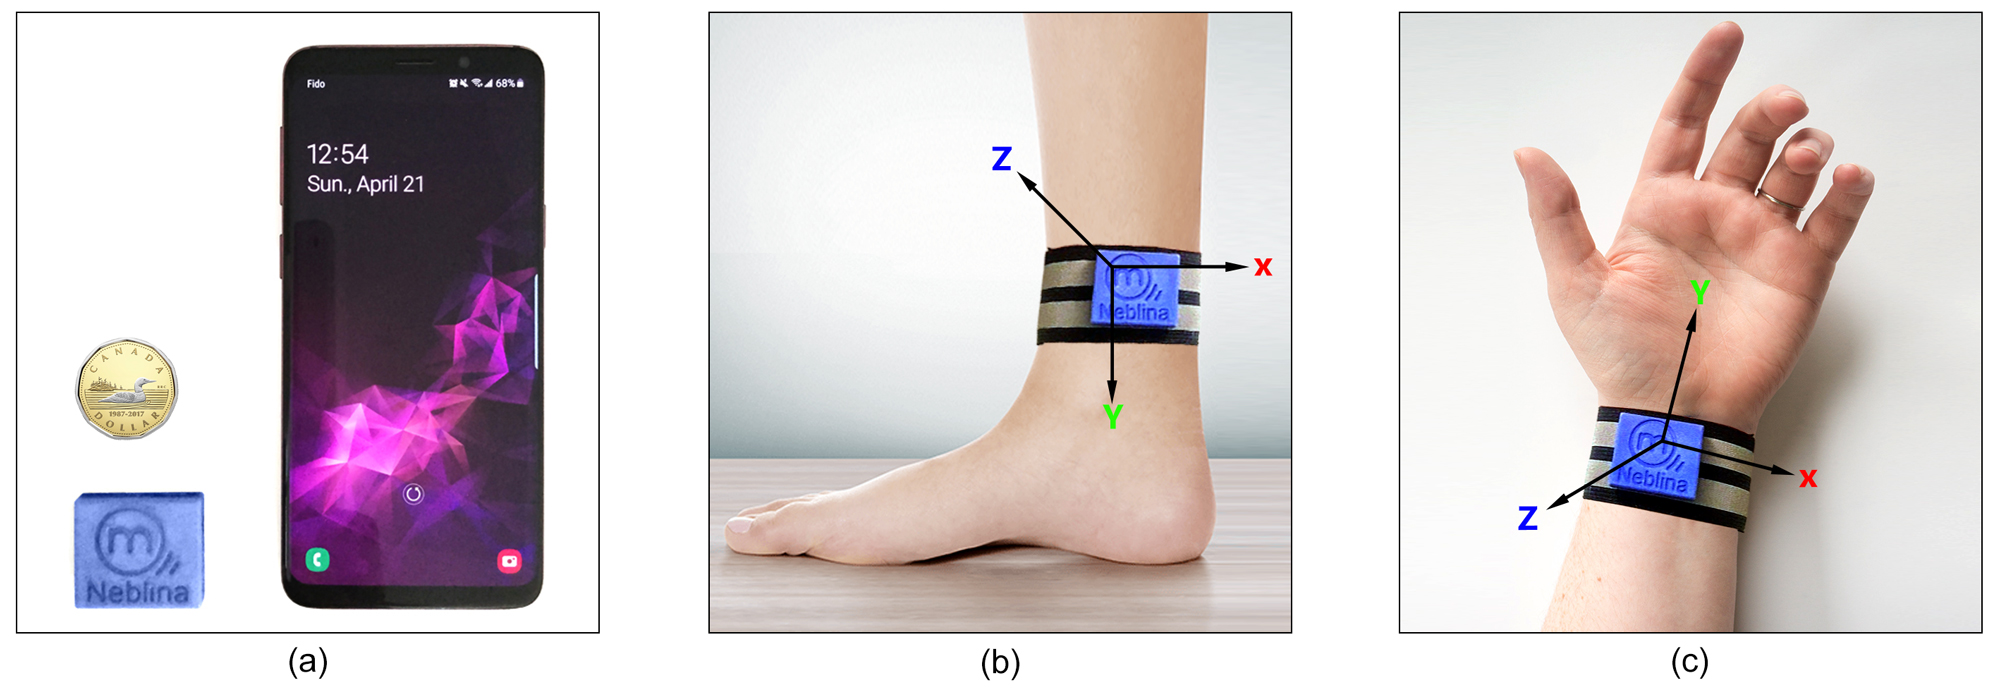
\includegraphics[width=10 cm]{Definitions/images/neblina_setup.jpg}
	\caption{Neblina setup. (a) Compares dimensions of Neblina with a 1 dollar coin and a cellphone (Sumsung Galaxy s9). (b) How Neblina located on foot using a strap. (c) How Neblina located on wrist using a strap.}
	\label{neblina_setup}
\end{figure} 

Although the device provides the magnetometer signals, we limited our process on using the accelerometer and gyroscope signals only. It is because the magnetometer signal can be affected by getting close to iron equipments in the gym. The frequency rate is fixed on 50Hz. It is worth to mention that the frequency rate more than 50Hz is not necessary because according to the Nyquist theorem~\cite{mazo1975faster}, this rate is enough to record a repetitive activity with 25 cycle per second which is so much faster than the iterations of normal workouts in the gym (one iteration per 1-5 seconds).

\subsection{Dataset}
In this section, we explain the process of preparing our dataset for experiments.

\noindent \textbf{Labeling.} In order to train a HAR model in a supervised machine learning process, we need labeled data points. Quality of labeled data points at this level has a direct impact on model performance ~\cite{janidarmian2017comprehensive}. In this study, 
to label the data we employed a process including three phases: (1) \textbf{By participant}: before beginning of each session, each subject was asked to fill a form about list of activities, number of sets, and the weights if applicable. (2) \textbf{By supervisor}: during the session, a supervisor manually records type of exercise, the moment of start and stop, and number of repetitions. (3) \textbf{By visual signal}: after finishing the session, in order to have our desired accuracy in labeling, we visually trace the signals of accelerometer and gyroscope to refine the regains assigned to each exercise. Using this way, any error missing in one step, will be caught in the next step.

\noindent\textbf{Adapting.} In order to make the dataset suitable for the experiments of this study, we trimmed the dataset. As we will explain later in \textit{Method} section, addition to k-fold cross-validation, we have two other evaluation methods including \textit{cross-session validation} and \textit{cross-subject validation}. These two additional evaluation methods bring some restrictions on the dataset. While \textit{cross-session validation} requires some activities to be repeated in several sessions, \textit{cross-subject validation} requires them to be repeated by several subjects. In addition, in RQ3, we want to compare results of different evaluation methods; Therefore, we have to use equal dataset for all evaluation methods. This is to say that for each activity to be suitable for this study, it should be repeated at least in certain number of sessions and also performed at least by certain number of subjects.
Table \ref{dataset_statistics} shows the statistics of the dataset after applying the restrictions. Column \textit{Sessions} shows the total number of sessions that an exercise appeared in. Column \textit{Subjects} shows how many subjects performed an exercise.
\begin{table}[H]
	\caption{Statistics of the dataset divided by type of exercise along with the experiments that involve them in.}
	\centering
	%% \tablesize{} %% You can specify the fontsize here, e.g., \tablesize{\footnotesize}. If commented out \small will be used.
	\begin{tabular}{ccccc|cc}
		\toprule
		\textbf{Exercise} & \textbf{Subjects} & \textbf{Sessions}	 & \textbf{Reps} & \textbf{Data Point}& \textbf{Body Involved}	& \textbf{Code}  \\
		\midrule		
		Lat Pull Down& 6& 22& 218& 14700& upper 		& A1\\
		Bench Press	& 6& 26& 273& 23230& upper 			& A2\\
		Biceps curl	& 4& 13& 115& 16095& upper			& A3\\
		Push-ups & 5& 16& 181& 9200& upper			& A4\\
		Treadmill& 4& 5& +1200 & 68780& Entire 			& A5\\
		Ab crunch machine& 4& 12& 108 & 10580& Entire & A6\\
		Crunch Twist &  3& 12& 98& 8760& lower			& A7 \\
		Russian Twist & 3& 8& 67& 8520& lower			& A8\\
		\bottomrule
	\end{tabular}
	\label{dataset_statistics}
\end{table}

%\begin{table}[H]
%	\caption{List of exercises along with target body part involved in each exercise. \diego{You mention our dataset contained 55 exercises. Is this just a sample?}}
%	\centering
%	%% \tablesize{} %% You can specify the fontsize here, e.g., \tablesize{\footnotesize}. If commented out \small will be used.
%	\begin{tabular}{ccc}
%		\toprule
%		\textbf{Exercise}	& \textbf{Body Involved}	& \textbf{Code}\\
%		\midrule
%		Lat Pull Down		& upper 		& A1\\
%		Bench Press		& upper 			& A2\\
%		Biceps curl		& upper			& A3\\
%		Push-ups & upper			& A4\\
%		Treadmill		& Entire 			& A5\\
%		Ab crunch machine		& Entire & A6\\
%		Reverse Crunch & lower			& A7 \\
%		Russian Twist & lower			& A8 \\
%		\bottomrule
%	\end{tabular}
%	\label{activity_list}
%\end{table}


\section{Method}
In this section, we explain the procedure of HAR as it is provided in Figure \ref{fig:main_approach}.

\subsection{Feature Extraction}
\label{sec:feature_extraction}



In literature, in order to gain more information from the sensory data (signal), the authors came up with hundreds of hand-crafted features among time domains, frequency domain or a combination of them ~\cite{wang2019survey}. Particularly, a feature highlights some specified signal attributes. Since in pattern recognition models, there are multiple features utilized by the model, an attribute might be redundantly presented several times through multiple features which results in increasing the computational cost and decreasing the model's performance.



In this study, we targeted five state-of-the-art sets of hand-crafted features. Table \ref{features_table} shows 31 functions along with a description/intuition about each one. Functions are grouped into sets (first column). Each set of functions is uniquely representative of a certain aspect of the signal.
 
\noindent\textbf{Preprocessing.} We used two tri-axial sensors (accelerometer and gyroscope) on two body positions (wrist and foot); So, To reproduce features, we normally apply these 31 functions on 12 raw signals coming from sensors. However, in some cases, an extra preprocessing operation is also required which will be explained in related section. Addition to this, to ensure that the data from different resources (sensors) are at the same scales, we performed a scale normalization in advance of any other computations.
\begin{table}[H]
	\caption{Statical Functions along with the definitions and abbreviations }
	\centering
	%% \tablesize{} %% You can specify the fontsize here, e.g., \tablesize{\footnotesize}. If commented out \small will be used.
	\begin{tabular}{p{0.9cm}p{5cm}p{7cm}p{1.3cm}}
		\toprule
		\textbf{Code} & \textbf{Function} & \textbf{Description/Intuition} & \textbf{{\scriptsize abbreviation}} \\
		\midrule
		{\footnotesize S1}&Minimum & {\scriptsize The value of the least sample}& MIN\\
		S2&Maximum & {\scriptsize The value of the greatest sample}& MAX\\
		{\footnotesize S3, SS8}&Mean&  {\scriptsize The average of all samples}& MEA\\
		{\footnotesize S4}&Median&  {\scriptsize The middle value of samples}& MEA\\
		{\footnotesize S5}&{\footnotesize Mean Absolute Deviation}& {\scriptsize The average distance between each sample and the mean of the stream}& MAD\\
		{\footnotesize S6}&{\footnotesize Median Absolute Deviation}& {\scriptsize The average distance between each sample and the median of the stream}& MAA\\
		{\footnotesize S7}&Inner Quartile Range  & {\scriptsize The amount of spread in the middle part \%50 of the stream}& IQR\\
		{\footnotesize S8}&Mean Crossing Rate& {\scriptsize The rate of passing the mean along the stream}& MCR\\
		{\footnotesize S9, SS9}&Standard Deviation& {\scriptsize how far the samples are from the mean}& SD\\
		{\footnotesize S10, SS10}&Variance& {\scriptsize the average degree of distance between samples and mean}& VAR\\
		{\footnotesize S11, SS11}&Root Mean Square& {\scriptsize The square root of the arithmetic mean of the squares of samples}& RMS\\
		{\footnotesize HB}& Histogram Bin&{\scriptsize a 20 bins distribution of data } & Hbin (1-20) \\
		{\footnotesize SS1}&Number of auto-correlation peaks& {\scriptsize The bigger number means non-periodic activity while smaller number refers to periodic activity }& NAcP\\
		{\footnotesize SS2}&Prominent auto-correlation peaks&{\scriptsize NAcP with an extra condition that the peaks should be greater than neighbours with at least a certain distance} & NAcPP \\
		{\footnotesize SS3}&Weak autocorrelation peaks&{\scriptsize NAcP with an extra condition that the distance between the peaks and neighbours should be less than a certain distance} & NAcWP \\
		{\footnotesize SS4}&Maximum autocorrelation value&{\scriptsize Value of the greatest peak (except for the initial peak at zero lag)} & MAXAc \\
		{\footnotesize SS5}&Height of the first autocorrelation peak (after zero-crossing)&{\scriptsize less height refers to more fluctuations within the stream  } & FAcP \\
		{\footnotesize SS6}&Power bins (10 bins)&{\scriptsize A 10 bins distribution of amplitudes of frequencies from 0.2-25Hz    } & Pbin(1-10) \\
		{\footnotesize SS7}&Integrated RMS&{\scriptsize The root-mean-square amplitude of the signal after cumulative summation } & IRMS \\
		Ph1&Movement Intensity&{\scriptsize the Euclidean norm of the total acceleration vector after removing the static gravitational acceleration } & MI\\
		Ph2&Normalized Signal Magnitude Area&{\scriptsize the acceleration magnitude summed over three axes within each window normalized by the window length } & SMA \\
		Ph3&Eigenvalues of Dominant Directions&{\scriptsize The eigenvectors of the covariance matrix of the acceleration data correspond to the dominant directions along which intensive human motion occurs.} & \\
		Ph4&Correlation between Acceleration along Gravity and Heading Directions&{\scriptsize It shows the human movement is either vertically or horizontally. } &CAGH \\
		Ph5&Averaged Velocity along Heading Direction&{\scriptsize The Euclidean norm of the averaged velocities along y and z axes over the window.} &AVH \\
		Ph6&Averaged Velocity along Gravity Direction&{\scriptsize averaging the instantaneous velocity along the gravity direction at each time t over the window } & AVG \\
		Ph7&Averaged Rotation Angles related to Gravity Direction&{\scriptsize The cumulative rotation angles around gravity direction} & ARATG \\
		Ph8&Dominant Frequency&{\scriptsize The frequency corresponding to the maximum of the squared discrete FFT component magnitudes of the signal from each sensor axis} & DF \\
		Ph9&Energy&{\scriptsize The sum of the squared discrete FFT component magnitudes of the signal from each sensor axis} & ENERGY \\
		Ph10&Averaged Acceleration Energy&{\scriptsize The mean value of the energy over three acceleration axes} & AAE \\
		Ph11&Averaged Rotation Energy&{\scriptsize The mean value of the energy over three gyroscope axes. } & ARE \\
		OI1&Orientation Independent&{\scriptsize result of applying PCA on Single Value Decomposition  of x/y/x values of the stream } & PCASVD(1-30) \\
		%		&&{\scriptsize } & \\
		%		&&{\scriptsize } & \\
		%		&&{\scriptsize } & \\
		\bottomrule
	\end{tabular}
	\label{features_table}
\end{table}


\subsubsection{Set\_A: Statistical Features (ST\_Set)}
Statistical features have been intensively investigated in different applications and proved to be effective and useful for HAR~\cite{rosati2018comparison}. These features are based on a comprehensive and intuitive understanding of how a given activity produces a set of discriminative features from measured sensor signals. We created a set of 264 features obtained by applying 11 statistical functions on 24 input signals, including (x/y/z axes of accelerometer and gyroscope, along with the cumulative sums of each axis). Functions are used in the statistical feature set are indicated by the code S1-S11 in Table~\ref{features_table}. 

\subsubsection{Set\_B: Histogram bins Features (HB\_Set)}
The second set of features are based on histogram representation of time series signal. Mathematically speaking, histogram representation of a signal is the probability distribution of signal over a period of time (often referred to as window size)~\cite{zardoshti1995emg}. In HAR, considering the fact that each activity contains a set of small movements (as small as one sample) with certain acceleration and rotation, histogram bins indicate the difference between activities by showing the different distributions of those small movements. Shirahama et. al.~\cite{shirahama2016codebook} used a histogram-based feature set for HAR. Comparing with statistical features, histogram bins have a significantly lower cost in terms of required processing time and memory usage~\cite{Sarbishei2019platform}. However, they are sensitive against the resolution/granularity of bins (count and width of bins). Following prior work~\cite{xi2017evaluation}, in this work, we consider 21 bins for values between 0 through 1 of a signal. Histogram bins are indicated with the code HB in Table~\ref{features_table}.

\subsubsection{Set\_C: Self-Similar Features (SS\_Set)}

Considering that an exercise activity is inherently more repetitive rather than a non-exercise activity, having a featureset that can capture the repetitive behaviour of signal is helpful. Morris et al. presented a featureset designed based on the idea of extracting repetitions forms of signal \cite{morris2014recofit}. These features can be extracted by: 1) Calculating the convolution of a signal with a shifted version of itself (auto-correlation) or 2)Extracting the components of the signal in the frequency domain. We extracted a number of self-similar features from our data, as shown in~Table~\ref{features_table}, features with code SS1-SS11. SS6 composed of 10 features per se; Thus, in total there are 20 functions.
There is a preprocessing operation required for this featureset. We transformed 3 input signals from each sensor (x/y/z inputs) to 4 processed signal describing as follows: 1) The magnitude of a/y/z axes, 2) The first principal component of all axes. 3) The first principal component of x and z axes. 4) The scaled normalized of y axis. It is important to mention that in our experiments, the y axis of sensor is along the user's arm. To build the featureset, we applied 20 functions on 16 processed signals. Therefore, this featureset contains 320 features.

\subsubsection{Set\_D: Physical Features (PH\_Set)}
One intuitive idea to design a set of features from sensory data is to take the principles of human movements into consideration. In 2011, Zhang et. al. ~\cite{zhang2011feature} introduced a set of features based on physical parameters of human motion. To have a strong physical meaning of motion data (e.g., moving forward, backward), they assumed that the sensor position and direction are known during the experiment. In other words, this types of features is derived based on the physical interpretations of human motion, called physical features. Comparing with other featuresets, these features are made up of a fusion of multiple sensor inputs rather than just one inputs sensor. In our paper, this featureset contains 11 features, labeled with the code Ph1-Ph11 in Table~\ref{features_table}. As a part of our pre-processing operation, we remove gravity from acceleration using gyroscope data by applying the method described in~\cite{Accelero5:online}.

\subsubsection{Set\_E: Orientation Independent Features (OI\_Set)}
In contrast to physical features, which depend on the position and orientation of sensors, Yurtman et. al~\cite{yurtman2017activity} proposed features that do not rely on variation of sensor orientation. In fact, in their model, they introduced Orientation-invariant transformations (OITs). They compared their model with the ordinary model - pre-defined sensor orientation, on five different datasets. Although their featureset did not have a significant impact on performance, it brought an extra added value to the model that lets it to be more robust against orientation. The OIT that they have introduced in their work is inspired by the idea of \textit{single value decomposition}\cite{moon2000mathematical}. Therefore, to create this featureset, first, we project every data point from original x/y/z space to a new space with same number of dimensions but at the farthest distance between data points. The intuition here is that the direction of the axes are defined by value of the data points not by x, y or z direction. Next, we apply PCA on the transformed data and take the first 30 most informative features \cite{janidarmian2017comprehensive}. In Table~\ref{features_table}, these type of features  are indicated by "OI" prefix.

\subsection{Activity Recognition}
\label{method}
In this paper, to discriminate the classes (exercises), we implemented four state-of-the-art classifiers on every featureset. The classifiers are implemented on mobile phones in various studies ~\cite{morris2014recofit,baldominos2019comparison,rosati2018comparison}: Support Vector Machine , Decision Tree, K-nearest neighbor, and Feed-forward neural network. 
\begin{table}[H]
	\caption{Classifier names along with hyper-parameters in this study}
	\centering
	\begin{tabular}{p{2cm}p{7.7cm}}
		\toprule
		\textbf{Classifier} & \textbf{Hyper-Parameters} \\
		\midrule
		SVM &  kernel = polynomial. degree = 3. gamma = 1/(data dimension)  \\
		\midrule
		KNN & K = 64. Similarity Method = Euclidean distance  \\
		\midrule
		FNN & { 2 dense layers with total 1000 and 400 units ~\cite{nair2010rectified}. One dropout layer (rate 60\%). Optimizer = Adam. learning rate = 0.0001. decay = 1e-10. 100 epochs.}\\
		\midrule
		DT & minimum split = 20, min number of sample in leaves = round(minimum split/3), maximum depth = 30 \\
		\bottomrule
	\end{tabular}
	\label{classifier_hyper_parameter}
\end{table}

\subsubsection{Support Vector Machine}
A multi-class Support Vector Machine (SVM) has been employed extensively in previous studies in HAR to discriminate among the activities~\cite{zhang2012physical,rosati2018comparison,morris2014recofit}. Morris et al.~\cite{morris2014recofit} showed that SVM provides higher accuracy in HAR. Assuming each data point is a co-ordinate (support vector) of feature space, the Support Vector Machine (SVM) is a method to find an optimum hyperplane with respect two some support vectors in order to separates different classes. 

% More Details: This happens at the expense of increasing the tolerance(mis-classification) of the model (loss function). In a situation that finding a hyperplane between two classes is impossible, the SVM project the feature space to another space having more number of dimensions. This is the responsibility of a function called Kernel function.


\subsubsection{Decision Tree}

Decision Tree is an ensemble method that provides an explainable model in classification. It is suitable for running on mobile phones with reasonable recognition performance \cite{mortazavi2014determining, baldominos2019comparison, shoaib2016complex}. Baldominos et al. \cite{baldominos2019comparison} reported the best recognition performance for decision tree among a set of classifiers including Naive Bayes, KNN, FNN, and Logistic Regression.\\
In order to distinct activities, decision trees look through every possible split in a range of values of a given feature and pick the best split between two adjacent points; The goal is that, after each split, branches become more "pure" (i.e., homogeneous activities) ~\cite{bishop2006pattern}. The "information gain" is a metric which assess error after each split. Thus, decision trees pick splits to maximize "Information Gain". There are two methods to assess the information: 1) Entropy and 2) Gini index.\\
Following ~\cite{rosati2018comparison, masum2018human}, we used the Gini index error metric.
There is also other hyper-parameters to control additional splits including maximum depth, minimum samples in leaves, and maximum number of leaf nodes. The values for these parameters are mentioned in Table \ref{classifier_hyper_parameter}. 

\subsubsection{K-nearest neighbor}
Another widely used classifier in HAR is the KNN algorithm ~\cite{wang2019survey,shakya2018comparative}, which works based on the calculation of the distance between data-points. As a lazy learning algorithm, KNN does not need off-line training. In other words, during the classification phase, for a given test data point, KNN finds the first \textit{k} nearest neighbors among training data-points. The majority of neighbors produces the classification output. Prior works showed that increasing k improves the performance on HAR model~\cite{kose2012online}. All the parameters for KNN in this study are mentioned in Table \ref{classifier_hyper_parameter}.

\subsubsection{Forward Neural Network}
By choosing a proper featureset, convention machine learning models (e.g., SVM, KNN) can achieve a good performance in activity recognition. However, we can improve it by using Deep Neural Network, which underlies the complementary information learned within the layers \cite{chen2018distilling}.
Recently, a number of studies have shown that Feed-forward Neural Networks achieve high performance in HAR\cite{chen2018distilling, zhu2009human}. A FNN is made up of a set of neurons, connected by weighted arcs, that process the input information:

\begin{equation}
\label{fnn_formula}
 y = f(\sum_{i}^{}w_{i}.x_{i})
\end{equation}
where y is the output of the neuron, $ w_{i} $ are weights of the incoming connections, $ x_i $ are inputs to the neuron, and $f$ is called transfer function and is selected according to the classification problem \cite{zhang1999geometrical}. Neurons in a FNN are organized in layers. Number of neurons at first layer and last layer are corresponding with number of features and number of activities, respectively~\cite{baldominos2019comparison}. Between input and output layers a certain number of hidden layers can be inserted, whose dimensions are usually decided testing different configurations ~\cite{baldominos2019comparison}. The configuration details of the network described in Table \ref{classifier_hyper_parameter}.

\subsection{Evaluation}
To evaluate the performance of the model, we need to split data into training and testing sets. For this purpose, in the context of HAR, there are traditional techniques such as k-fold cross-validation, leave-one-subject-out~\cite{jordao2018human}, as well as, the relatively less common techniques like leave-one-trial-out~\cite{sena2018multiscale}. In this study, we used all three validation methods while we modified leave-one-trial-out to leave-one-set-out in order to make it more flexible for repetitive activities. 

\subsubsection{K-fold Cross validation}
The most typical approach to evaluate the performance of HAR model is k-fold-cross validation. The idea is to use resampling procedure in a way that all the samples be used once during the testing period, mostly in the case of having limited dataset. The so called parameter k refers to the number of groups that the given dataset is to be split into. Each time one group becomes the test set and remaining $k-1$ groups become training set. During k turns, we evaluate the model k times on different test set and train set. Finally, the performance is summarized by averaging the performance of all k turns. In this work, we apply k-fold cross validation on all the models. That is, the dataset breaks down equally into 10 parts (folds). During 10 iterations of evaluation, every part is considered as test-set and remaining parts as train-set. 
%\diego{Is the k-fold stratified? That is, do you guarantee a homogeneous distribution of classes while splitting the data into k groups?} Hosein: This is an interesting point that we may mention in it cross-subject and cross-trial because they are not homogeneous necessarily.
\subsubsection{Leave-One-Subject-Out Cross validation}
Leave-One-Subject-Out (LOSO) validation is a special case of cross-validation, where a subject can be seen as a fold, hence, the number of subjects determine the number of folds. Furthermore, the LOSO validation technique reflects a realistic scenario, where a model is trained in an offline way, using the samples of some subjects, and is tested with samples of unseen subjects. It is important to note that using LOSO may present high variance in performance from one subject to another, since the same activity can be performed in different ways by the subjects. 

\subsubsection{Leave-One-Trial-Out Cross validation}
The Leave-One-Trial-Out (LOTO) cross validation is similar to LOSO, however, instead of considering the subjects as folds, each trial (session) of doing the activity is considered as a fold. In fact, sessions might belong to same subjects of different subjects. To implement LOTO, on dataset of each subject which may contain several sessions, we assigned an index to each session. So, in order to split the dataset into test and train, we use session id instead of subject id in LOSO. The main advantage of using this method comparing with LOSO is that it needs a smaller number of subjects since each subject can have several sessions. In addition, similar to LOSO, this method does not suffer from having same content between train set and test set.\\

\noindent \textbf{Measurements.} Most commonly used measures to asses the performance of a HAR model in prior works are: accuracy\cite{brownlee2018gentle,zhang2011feature,mehrang2017human} and F-measure\cite{rosati2018comparison,Nourani_CoMoRea2019}. We used accuracy and F1. Using F1 is essential since our dataset is imbalanced. Thus, since F1 relies on both the precision and recall, it is less affected by imbalanced dataset. Specifically, measurement units in this study determined as follows:
\begin{itemize}
	\item \noindent \textbf{Accuracy} measures how often the classifier is correct. Specifically, it is equal to (TN + TP) / total.
	%\item \noindent \textbf{Miss-classification} measure how often the classifier is incorrect. Specifically, it is equal to (1 - Accuracy).
	%\item \noindent \textbf{Precision} measures when the classifier detects an activity, how often it is  correct. Specifically, it is equal to TP / (TP + FP). 
	%\item \noindent \textbf{Recall} measures when user is doing a certain activity, how often the classifier can detect it correctly. Specifically, it is equal to TP / (TP + FN). This term is also known as \textit{Sensitivity} or \textit{True Positive Rate}.
	\item \noindent \textbf{F-Score} measures a weighted average of both Recall and Precision. Specifically, it is equal to (2 x Precision x Recall ) / (Precision + Recall). 
	%\item \noindent \textbf{Null Error Rate:} measures how often it is incorrect if we constantly return the major class in dataset as response of the classifier. To the best of our knowledge, in most HAR datasets, the major class is non-activity class.
\end{itemize}

Where:
\begin{itemize}
	
	\item \textbf{True Positive (FP):} These are cases in which we predict an activity, and user was doing that activity.
	
	\item \textbf{True Negative (TN):} Is where we predict a non-activity period, and user was not doing a certain activity.
	
	\item \textbf{False Positive (FP):} Is where we predict a certain activity for a segment of data, however, user is either doing another specific activity or generally doing something else (out of activity given list).
	
	\item \textbf{False Negative (FN):} Is where we predict either a not-activity period or a certain activity, but, it is not the activity that user is really doing that.
	
\end{itemize}

\section{Results}
Our study aims to perform a systematic examination on HAR pipeline (Figure \ref{fig:main_approach}) through three crucial steps. First, in RQ1, we compare different featuresets and indicate the one providing the best recognition performance; Next, using this featureset as input, we examine four classifiers in classification phase to find the model with highest performance (RQ2). Finally, in RQ3,  we target the impact of different evaluation methods on performance of our model.

\subsection{RQ1: Which featureset provides the best performance in HAR?}

As motivated earlier, choosing an appropriate featureset significantly impacts on recognition performance. Many different featuresets have been presented in previous works. While they all are reporting remarkable performances on HAR, they can not be compared with each other due to different experimental setups that those results are achieved. Hence, we aim to investigate five state-off-the-art featuresets when all other factors (i.e., dataset, classifiers) are fixed. Each featureset is examined by four classifiers including FNN, KNN, SVM, and DT. To measure the performance, we used 10-fold cross validation and F-score metric for each experiment.

Table \ref{f1_classifier_featureset} shows the performance for each featureset (columns 2-6) on different classifiers (rows 2-5). We highlighted the best performance for each featureset in the Table. It can be seen that the best performing featuresets are \textit{statistical featureset} (ST\_Set) and \textit{Histogram bins} (HB\_Set), achieving approximately 95\% of F1. However, the remaining featuresets have never exceeded 90\% of F1. The highest recognition performance for \textit{self-similar featureset}, \textit{physical featureset}, and \textit{Orientation independent featureset} are respectively 89.18\%, 85.34\%, and 78.47\%.

It is worth mentioning here that regarding th computational cost of featuresets, \textit{histogram bins} is placed at the lowest complexity (cost) with having only $ O(n\log m) $ where \textit{m} is number of bins. \textbf{Low computational cost along with providing the highest recognition performance make \textit{histogram bins} an ideal candidate featureset for Wearables, since they are limited in resources}. 
On the other hand, \textit{Orientation Independent} features achieved the minimum performance (77.44\% on average). Although it reached to a relatively lower performance among featuresets, it allows for a flexibility in the way that sensors are placed on a subject.

%classifiers have almost similar behaviour over different featuresets. Almost all classifiers on \textit{statistical featureset} and \textit{Histogram bins} deliver their higher performance which means these two featuresets bring the most informative features rather others. While almost in all featuresets, models are exceeding 80\% accuracy, the orientation invariant features provides insufficient information for successfully tackling activity recognition, since the accuracy never exceeds 77\%. \textbf{Interestingly, the Histogram Features with having the least complexity in computation gained the best performance among other featuresets at 95.89\% when using FNN and 93.30\% on average among all classifier.} In fact, accuracy achieved by the top-performing models (FNN and SVM) are significantly better when they use histogram features. This might happen due to choosing an appropriate bin width based on length of activity and windows size.\\
%We naturally expect the accuracy achieved with the Orientation Invariant featureset to be lower compared to the other featureset since other featuresets (especially physical features) know about the directions of moving and gravity. However, the goal in creating this featureset was to provide the user the flexibility to place the sensor units at any orientation while this ability is not available on other featuresets. 

\begin{table}[H]
	\caption{F-score for each classifier over different feature-sets using 10-fold cross validation }
	\centering
	\begin{tabular}{p{2cm}p{1.7cm}p{1.7cm}p{1.7cm}p{1.7cm}p{1.7cm}p{1.7cm}}
		\toprule
		\textbf{Classifier} & \textbf{ST\_Set} & \textbf{HB\_Set} & \textbf{SS\_Set} & \textbf{PH\_Set} & \textbf{OI\_Set} & Average \\
		\midrule
		SVM &  94.98\% & 94.55\% &\cellcolor{gray!35}{89.18\%} &84.15\% & \cellcolor{gray!35}{78.47\%} &87.82\%\\
		KNN & 91.50\% & 90.21\% & 85.61\% &81.93\% & 76,41\%& 85.50\% \\
		FNN & \cellcolor{gray!35}{95.31}\% & \cellcolor{gray!35}{95.89\%} &  87.93\% &\cellcolor{gray!35}{85.34\%} & 77.59\% & \cellcolor{gray!35}{88.29}\%\\
		DT & 88.64\% & 89.18\% &  82.94\% &79.37\% & 74.02\% &82.83\%\\
		\bottomrule
		\textbf{Median} & 92.36\% &  92.92\% &86.41\% & 82.70\% & 77.12\%&86.30\%\\
		\midrule
		\textbf{Average} & 92.74\% &  \cellcolor{gray!35}{93.30\%}  & 86.77\% &83.04\% & 77.44\% &86.66\%\\
		\bottomrule
	\end{tabular}
	\label{f1_classifier_featureset}
\end{table}
%\begin{table}[H]
%\caption{F1 for each classifier and for all each feature-set using 10-fold cross validation }
%\centering
%%% \tablesize{} %% You can specify the fontsize here, e.g., \tablesize{\footnotesize}. If commented out \small will be used.
%%a = statistical - b=histogram - c=self-similar d=physical feature e=orientation independent
%\begin{tabular}{p{3cm}p{2cm}p{2cm}p{2cm}p{2cm}p{2cm}}
%	\toprule
%	\textbf{Classifier} & \textbf{Set\_A} & \textbf{Set\_B} & \textbf{Set\_C} & \textbf{Set\_D} & \textbf{Set\_E} \\
%	\midrule	
%	SVM & 72.33\% & 79.08\% & 67.14\% &66.45\% & 60.89\% \\
%	KNN & 60.17\% & 76.00\% & 73.23\% &57.12\% & 53.98\% \\
%	FNN & 80.71\% & 84.38\% & 66.10\% &66.13\% & 60.02\% \\
%	DT & 63.15\% & 67.99\% & 71.18\% &63.61\% & 60.33\% \\
%	\bottomrule
%\end{tabular}
%\label{f1_classifier_featureset}
%\end{table}

%\hosein{if we use the feature selection method to evaluate featuresets, so, One interesting question to ask is whether the features selected by feature selection methods are truly important for our activity recognition problem. To answer this question, we can first remove the top 50 features selected by feature selection methods. Then perform the same procedure to classify the activities. if the classification errors decrease significantly, This indicates that the top 50 features selected contain more important information than the remaining feature set.}

\subsection{RQ2: Which classifier performs better on gym exercise recognition?}

As we saw in RQ1, different classifiers perform differently even on same featureset. Hence, one question that we aim to answer is whether certain classifiers perform better than others. Therefore, in this research question we do an empirically comparison between the performance of different classifiers. We use four popular classifiers in HAR including SVM, KNN, FNN, and DT. It is important to mention that we evaluate the model using default configurations since the optimizing the classification is not a goal of this study. The default configuration used for each model is mentioned in \ref{method} section. From RQ1, we found \textit{histogram bins} as the most informative featureset. So, we use it for training model in this experience. The K-fold cross-validation with 10 folds is used for measuring classification results; Thus, we have 10 results of F-Score for each classifier. To compare results, we used \textit{Student t-test}.
Figure \ref{fig:classification_comparison} shows how results of each classifier are spread out over 10 rounds. FNN followed by SVM show a range between 85\% through 99\% of F-measure over 10 trials while DT and KNN are showing more divergence over trials respectively between (67\%-98\%) and (77\%-97\%) of performances. The mean for all classifiers are shown in Figure \ref{fig:classification_comparison}. Since the \textit{p-value} is 0.057 we can reject the null hypothesis, saying that with 93\% of confidence, the average performance showing in Figure \ref{fig:classification_comparison} is what exactly that those classifiers perform in practice. In other words, FNN and SVM with $95\% \pm <1\% $ are delivering highest performances whereas KNN and DT with 90.21\% and 88.29 of F-Scores respectively are giving lower performances.
\begin{figure}[H]
	\centering
	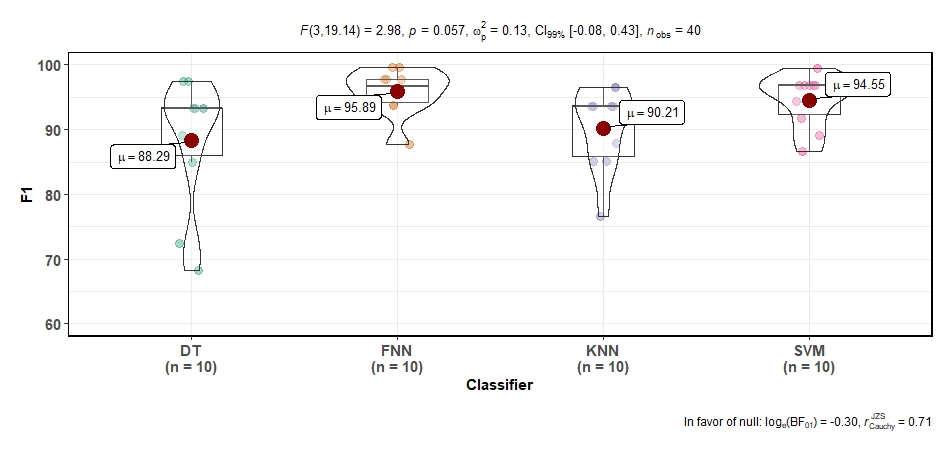
\includegraphics[width=14 cm]{Definitions/images/F1_results_vioPlot.jpeg}
	\caption{Comparison between the performance of classifiers}
	\label{fig:classification_comparison}
\end{figure}



\subsection{RQ3: How do different evaluation methods impact the reported HAR performance?}

K-fold is one of the most popular methods to evaluate the performance of a HAR model~\cite{wang2019survey}. However, in an empirical study, Jordao et al.~\cite{jordao2018human} showed that the result of k-fold cross validation can be biased when using sliding windows, a technique that is commonly used in HAR. Therefore, the focus of this research question is to asses models by two state-of-the-art evaluation methods namely, Leave-One-Subject-Out (LOSO) cross validation~\cite{liu2011multisensor} and Leave-One-Trial-Out (LOTO) Cross validation~\cite{sena2018multiscale,jordao2018human}. 

In K-fold, splitting the dataset (\textit{K}) is decided by researcher based on the size of dataset as well as the type of classification problem\cite{jordao2018human}. Table \ref{dataset_statistics} shows how the data is distributed for each activity. To split the dataset in each validation method based on number of activities and number of subjects.
However, in LOSO and LOTO, it also required to respect to the distribution of activities among number of participants, and sessions of each participant. In fact, an activity should appears at least in more than one session by same subject to be eligible for LOTO cross-validation. In this experiment, for LOSO we used data from 6 subjects while compromising some activities were missing for 2 subjects. For LOTO, we have employed the data of 8 sessions while some sessions belong to same person. For those activities that appeared in more than 8 sessions, we merged their sessions to each other. 

Figure~\ref{fig:evaluation_comparison} compares the performance of models using 10-fold cross validation (in blue), LOTO (in orange), and LOSO (in grey). As we can see from the Figure, for all featuresets and all classifiers, the evaluation technique impacts the reported performance. In fact, we see that in general, k-fold cross validation always provides better results than LOTO and LOSO. As mentioned earlier, due to the use of sliding windows in HAR, LOTO or LOSO are more realistic evaluation techniques and than k-fold cross validation. It can be seen that there is a significant distance between results of LOTO and LOSO (~10\%). This can be due to differently performing an exercise by different subjects in LOSO. However, in LOTO, since the model is trained by the data of at least one session of each subject it returns a better result. 

%For each classifier, results in the left columns have been obtained using 10-Fold evaluation, in middle columns using LOTO cross validation, and the right columns using LOSO cross validation. From the results, independent from featureset / classifier, it is obvious that the evaluating by LOTO or LOSO gives a lower performance (on average ~6\% and ~16\% respectively).
%Because of having an overlap between every consecutive data points due to using sliding window, a part of data which is used to generate a data point for train set will be used in data points for test set as well (96\% identical in this case). Therefore, We basically expect the performance achieved with k-fold to be higher than other methods because there is a significant correlation between train set and test set in this method. In other words, in K-fold, first, we generate data points from raw data (using sliding window), then, split them into test set and train set. However, in two other evaluation methods, training set and testing set are generated independently. So, the results are turned out from a less correlated test set thereby showing more realistic result, comparing with baseline. It can be seen that there is a significant distance between results of LOTO and LOSO (~10\%). This can be due to differently performing an exercise by different subjects in LOSO. However, in LOTO, since the model is trained by the data of at least one session of each subject it returns a better result. To compare classifiers, still FNN and SVM deliver the best result on all featuresets.

 
\begin{figure}[H]
	\centering
	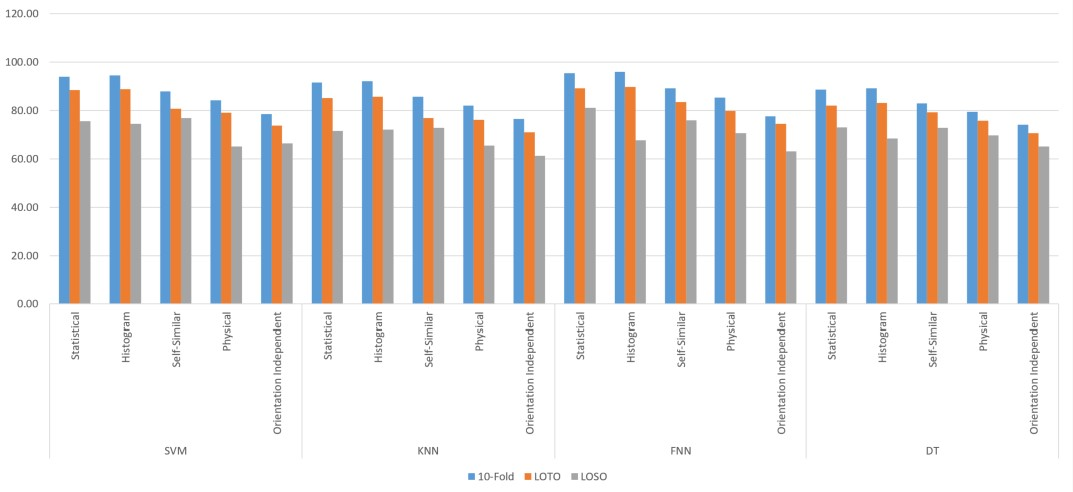
\includegraphics[width=14 cm]{Definitions/images/evaluation_comparison_2.jpg}
	\caption{Comparison between evaluation methods (10-Fold, LOTO, LOSO)}
	\label{fig:evaluation_comparison}
\end{figure} 
%
%\begin{table}[H]
%	\caption{F-Score for each classifier and for all each feature-set using Leave-One-Trial-Out cross validation }
%	\centering
%	\begin{tabular}{p{3cm}p{2cm}p{2cm}p{2cm}p{2cm}p{2cm}}
%		\toprule
%		\textbf{Classifier} & \textbf{Set\_A} & \textbf{Set\_B} & \textbf{Set\_C} & \textbf{Set\_D} & \textbf{Set\_E} \\
%		\midrule	
%		SVM &  \cellcolor{gray!35}{76.73\%} & 73.11\% & \cellcolor{gray!35}{76.70}\% &69.19\% & 62.13\% \\
%		KNN & 72.91\% & 75.58\% & 74.24\% &70.36\% & 61.74\% \\
%		FNN & \cellcolor{gray!35}{77.07}\% & \cellcolor{gray!35}{79.87\%} &  \cellcolor{gray!35}{76.06\%} &\cellcolor{gray!35}{73.04\%} & 66.60\% \\
%		DT & 69.48\% & 71.70\% & 72.58\% &71.18\% & 65.34\% \\
%		\bottomrule
%	\end{tabular}
%	\label{Table:LOTO_results}
%\end{table}
%
%\begin{table}[H]
%	\caption{F-Score for each classifier and for all each feature-set using Leave-One-Subject-Out cross validation }
%	\centering
%	\begin{tabular}{p{3cm}p{2cm}p{2cm}p{2cm}p{2cm}p{2cm}}
%		\toprule
%		\textbf{Classifier} & \textbf{Set\_A} & \textbf{Set\_B} & \textbf{Set\_C} & \textbf{Set\_D} & \textbf{Set\_E} \\
%		\midrule	
%		SVM &  \cellcolor{gray!35}{68.83\%} & 69.11\% & \cellcolor{gray!35}{76.70}\% &69.19\% & 62.13\% \\
%		KNN & 72.91\% & 75.58\% & 74.24\% &70.36\% & 61.74\% \\
%		FNN & \cellcolor{gray!35}{77.07}\% & \cellcolor{gray!35}{79.87\%} & 76.06\% &\cellcolor{gray!35}{73.04\%} & 66.60\% \\
%		DT & 69.48\% & 71.70\% &  \cellcolor{gray!35}{72.58\%} &71.18\% & 65.34\% \\
%		\bottomrule
%	\end{tabular}
%	\label{Table:LOSO_results}
%\end{table}


\section{Discussion}
\subsection{Performance of FNN}
In this section we focus on investigating the FNN model on Histogram bins more in detail. Figure \ref{fig:fnn_hbins_confusion_matrix} shows the normalized confusion matrix for FNN model on \textit{set\_B}. One can see that activities such as Lat Pull Down and Bench Press (A1 and A2) are classified more accurately than activities such as Crunch Twist (A7) which is misclassified as Russian Twist (A8). In other words, it can be said that activities of a similar nature are more willing to get misclassified. Especially when the subject is not experienced enough on performing the exercise, recognizing the activity get harder. Addition to this the class A0 which stands for non-exercise activity is misclassified 1 percent as almost all other classes. This could be a result of variation in the distribution of data for all classes. This can also be illustrated in Figure \ref{fig:fnn_hbins_confusion_matrix} where the performance at first row is distributed across all the classes. Because of the uniform nature of data distribution among all classes, and because of a balanced nature, similar activities could be classified more accurately.\\
\begin{figure}[H]
	\centering
	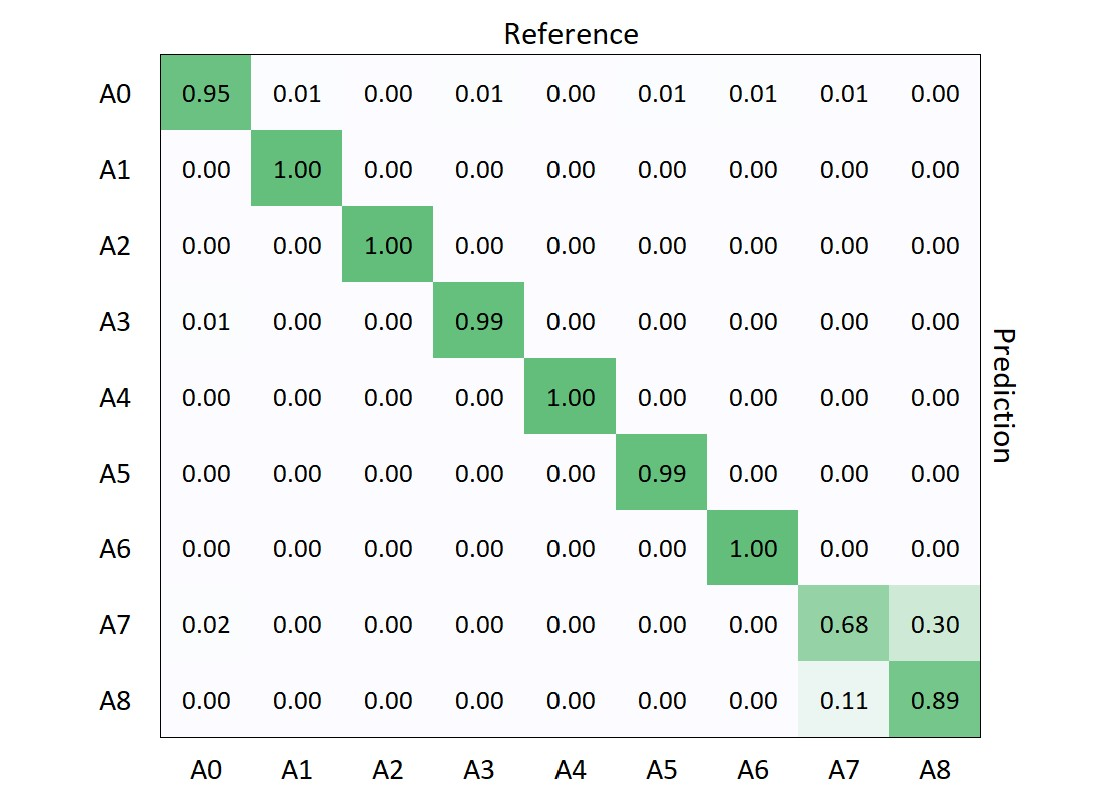
\includegraphics[width=7 cm]{Definitions/images/fnn_histogram_set.jpg}
	\caption{Normalized confusion matrix for FNN classifier using histogram dataset(set\_B). A0 in this table stands for non-exercise data points.}
	\label{fig:fnn_hbins_confusion_matrix}
\end{figure} 

%\hosein{Since we already mention this aspect in RQ3, we may want to remove this subsection:\\
%\subsection{K-fold Evaluation result is biased?}
%As we argued earlier, each process has a drawback that might cause a negative impact on the methods. For instance, SNOW can produce biased results and the FNOW generates few samples. To face these problems, we propose the Leave-One-Trial-Out (LOTO) sample generation process.
%From the literature, the most popular method to evaluate a HAR model is K-fold cross-validation. In this method the data splits into k equal parts. The k-1 parts go for training and one part left for test. This process repeats for each k, separately. Main aim of this method is to keep the test and train part separate from each other and use all the samples in train and test. However, in case of using the conventional sliding window (with n\% overlap) for generating data-samples it is impossible for samples to be completely separated from each other. It is because of the overlap period which is common between each two windows in a sequence. In other words, as mentioned in \cite{jordao2018human}, the result is always biased because n\% of the data are identical between test and train part. To avoid this drawback, a ordinary evaluation method is Leave-One-Subject-Out (LOSO). Basically, this method resembles the k-fold cross-validation in which a fold is replaced by a subject. This method is secure against being biased since the data from each subject has no common area with other subjects. However, in order to have the performance in a satisfactory level, we have to increase the number of subjects, respectively. The Leave-One-Trial-Out (LOTO) cross-validation\cite{jordao2018human} is similar to LOSO, but use the data of a trial instead of a subject. Thus, we have ensured that the samples are basically separated and the performance does not depend on the number of subjects any more.
%\hosein{+ showing it in a example}
%}
%\subsection{Hand-Crafted Features VS Automated Features}

%The extraction of hand-crafted features are computationally lightweight and efficient to implement especially in ubiquitous devices. In addition, they are easy to understand due to the physical meanings of the features and finally, they work well for many HAR problems. However, choosing the right feature may be challenging based on the type of the problem underhand and also extracting the appropriate set of features depends on domain knowledge. \\
%In recent years, in parallel with the advancement of deep learning in many fields such as speech recognition and natural language processing, Deep Learning (DL) approaches have been explored in HAR. While most conventional methods use hand-crafted feature extraction, DL performs automatic high-level feature extraction thereby relieving the effort on designing features. In fact, instead of extracting feature manually, we train a neural network with raw input data from sensor. The strength of the automatically learned features by the deep networks is that the learning can be very deep, and the learning process does not rely on domain knowledge. In terms of performance, to the best of our knowledge, although there are researchs on both models, there is no comprehensive comparison to show a DL model how much better than a model on  a given hand-crafted features.\\
%In this section, we setup an experiment to compare the performance of a state-of-the-art Convolutional Neural Network (CNN) with the performance of the best model achieved in RQ3. 
%The input to the neural network consists of the reshaped sensor data from multiple sensors. Considering 5-second sliding window with 0.2 second shifting size (same setup as RQ1). Considering 50Hz sampling rate and three axes for each of the accelerometer and gyroscope sensors of two Neblinas, in total for one input window (channel), we have a matrix with three dimensions (5 * 50 * 12). This means that we stack the sensors on top of each other in a single channel. Table \ref{Table:CNN_network} shows the architecture of the network.

%Results achieved from this experiment has been shown in Figure \ref{cnn_result}.
%\begin{figure}[H]
%	\centering
%	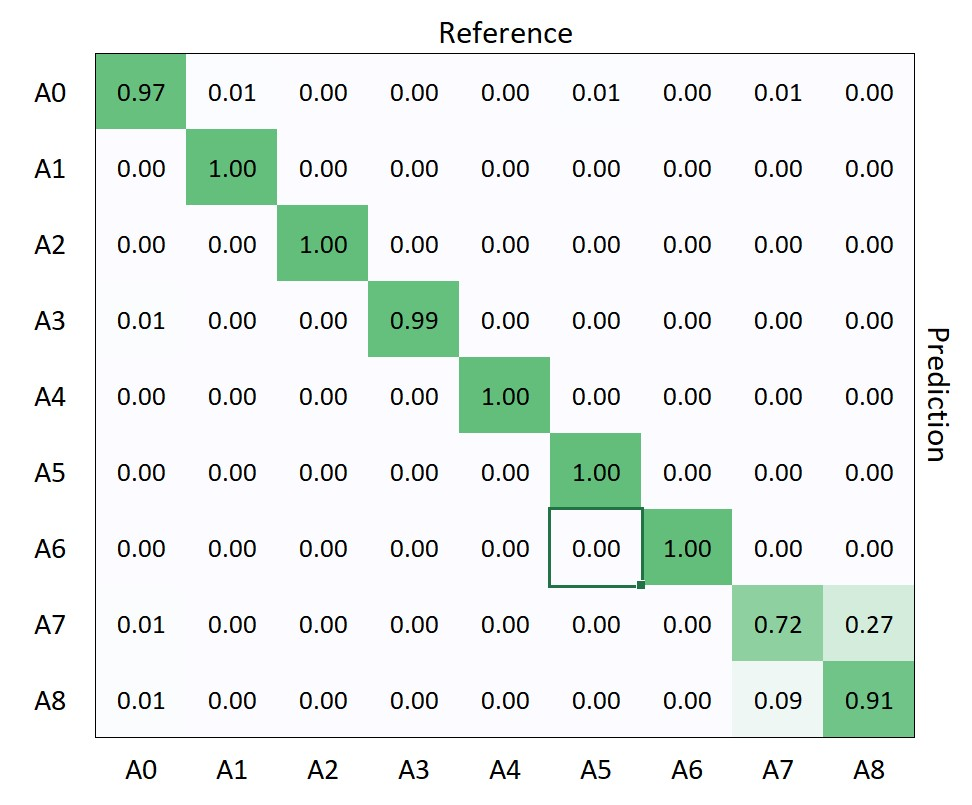
\includegraphics[width=7 cm]{Definitions/images/cnn_confusion.jpg}
%	\caption{Normalized confusion matrix for CNN classifier. A0 in this table stands for non-exercise data points.}
%	\label{cnn_result}
%\end{figure} 
%We evaluate the model using a 10-fold cross validation (same setup as RQ1). on average, the accuracy of the model in recognizing the activities is 96.11\% which is 0.22\% better than the best accuracy achieved by FNN model on histogram bins features. To investigate the performance of the model on  recognizing each activity, Figure \ref{cnn_results} shows the confusion matrix of the CNN model.

%\begin{table}[H]
%	\caption{Summary of the CNN model layers, output shape, and number of parameters }
%	\centering
%	\begin{tabular}{p{8cm}p{3cm}}
%		\toprule
%		\textbf{Layer} & \textbf{Value}  \\
%		\midrule	
%		Input shape &  250 * 12 * 1 \\
%		Convolutional filters CL1 &  100 \\
%		Kernel size CL1 &  (15, 3) \\
%		Strides CL1 &  (1, 3) \\
%		Convolutional filters CL2 &  25 \\
%		Kernel size CL2 &  (15, 18) \\
%		Strides CL2 &  (3, 1) \\
%		Convolutional filters CL3 &  75 \\
%		Kernel size CL3 &  (15, 18) \\
%		Strides CL3 &  (3, 1) \\
%		Convolutional filters CL4 &  75 \\
%		Kernel size CL4 &  (15, 18) \\
%		Strides CL4 &  (3, 1) \\
%		Convolutional filters CL5 &  25 \\
%		Kernel size CL5 &  (15, 18) \\
%		Strides CL5 & (3, 1)  \\
%		Activation function CL1, CL2, CL3, CL4, CL5 &  relu   \\
%		Dropout CL1, CL2, CL3, CL4, CL5 & 0.50 \\
%		DL1 neurons & 250  \\
%		DL2 neurons & 8 \\
%		Activation function DL2 &  softmax \\
%		
%		\bottomrule
%	\end{tabular}
%	\label{Table:CNN_network}
%\end{table}

%\hosein{we may want to mention: in most daily HAR tasks, those methods may heavily rely on heuristic handcrafted feature extraction, which is usually limited by human domain knowledge (Bengio, 2013) 
%Those work indicated that, when the HAR data is multi-dimensional and activities are more complex, more hidden layers can help the model train well since their representation capability is stronger (Bengio, 2013) }

\subsection{Learning Speed }
The last but not the least aspect worthy to mentioned is various converging speed of FNN between using different featuresets. As mentioned in RQ1, training an FNN on Histogram bins after 100 epochs delivers the best performance comparing with result of training at same number of epochs on other featuresets. In this section, we investigate velocity of FNN on reaching its best performance during first 100 epochs. Figure \ref{fig:fnn_learning_speed} shows the performance of FNN models using different featuresets. As we expect, after 100 epochs, the models on histogram bins, statistical features, self-similarity features have been reached a higher level of F1 (all above 90\%) while the had been stable almost after first 20 epochs. On the other hand, the trend for both models on physical features and orientation independent are below 90\% while they have not been stable even at greater number of epochs (close to 100). This is to say that FNN can be trained faster when it is feed with histogram bins, statistical features, or self-similarity features rather two other featuresets. Interesting, for FNN on histogram features, the first time to touch the best performance is at the 5th epoch. This number for models on statistical features and self-similarity features happens after 14 epochs and 12 epochs respectively.

\begin{figure}[H]
	\centering
		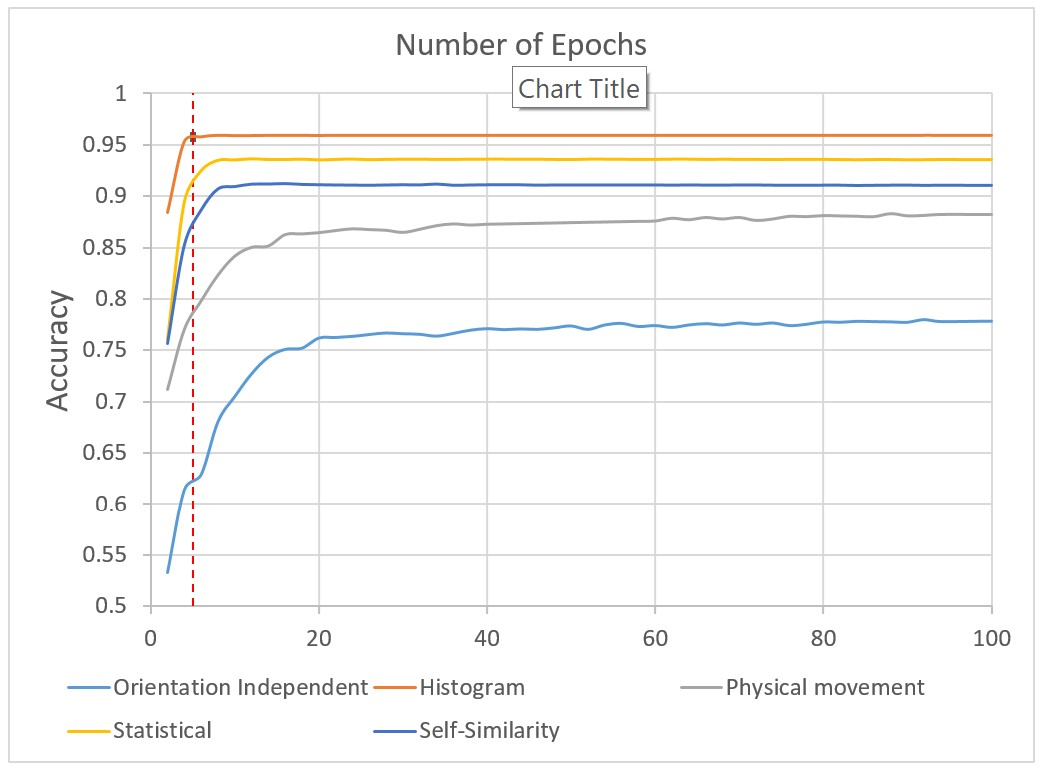
\includegraphics[width= 10cm]{Definitions/images/fnn_learning_speed.jpg}
		\caption{F-Score of FNN during first 100 epochs using 5 featuresets}
		\label{fig:fnn_learning_speed}
\end{figure} 


%%%%%%%%%%%%%%%%%%%%%%%%%%%%%%%%%%%%%%%%%%
\section{Conclusions}

Human activity recognition is an important research topic
in pattern recognition and pervasive computing. In this paper, we have studied on the state-of-the-art models using hand-crafted features and traditional models. From RQ1 and RQ2, it turned out that FNN and histogram bins can deliver a superior performance rather other 19 pairs of classifiers and featuresets. It is also important to mention that the number of bins and width of each bin play important roles on extracting informative features. In RQ3, comparing leave-one-trial-out cross validation with two conventional evaluation methods (k-fold and LOSO), we saw that LOTO and LOSO provide a more realistic result rather K-Fold at the expense of declining the performance. Addition to this, we figured out, LOTO can address two issues which are not solved LOSO, including: 1) it is applicable on datasets with less number of subjects comparing with LOSO which requires more subjects. 2) it can suppress the impact of performing differently of an exercise by different subjects. 

%%%%%%%%%%%%%%%%%%%%%%%%%%%%%%%%%%%%%%%%%%
\vspace{6pt} 

%%%%%%%%%%%%%%%%%%%%%%%%%%%%%%%%%%%%%%%%%%
%% optional
%\supplementary{The following are available online at \linksupplementary{s1}, Figure S1: title, Table S1: title, Video S1: title.}

% Only for the journal Methods and Protocols:
% If you wish to submit a video article, please do so with any other supplementary material.
% \supplementary{The following are available at \linksupplementary{s1}, Figure S1: title, Table S1: title, Video S1: title. A supporting video article is available at doi: link.}

%%%%%%%%%%%%%%%%%%%%%%%%%%%%%%%%%%%%%%%%%%
\authorcontributions{For research articles with several authors, a short paragraph specifying their individual contributions must be provided. The following statements should be used ``conceptualization, X.X. and Y.Y.; methodology, X.X.; software, X.X.; validation, X.X., Y.Y. and Z.Z.; formal analysis, X.X.; investigation, X.X.; resources, X.X.; data curation, X.X.; writing--original draft preparation, X.X.; writing--review and editing, X.X.; visualization, X.X.; supervision, X.X.; project administration, X.X.; funding acquisition, Y.Y.'', please turn to the  \href{http://img.mdpi.org/data/contributor-role-instruction.pdf}{CRediT taxonomy} for the term explanation. Authorship must be limited to those who have contributed substantially to the work reported.}

%%%%%%%%%%%%%%%%%%%%%%%%%%%%%%%%%%%%%%%%%%
\funding{Please add: ``This research received no external funding'' or ``This research was funded by NAME OF FUNDER grant number XXX.'' and  and ``The APC was funded by XXX''. Check carefully that the details given are accurate and use the standard spelling of funding agency names at \url{https://search.crossref.org/funding}, any errors may affect your future funding.}

%%%%%%%%%%%%%%%%%%%%%%%%%%%%%%%%%%%%%%%%%%
\acknowledgments{In this section you can acknowledge any support given which is not covered by the author contribution or funding sections. This may include administrative and technical support, or donations in kind (e.g., materials used for experiments).}

%%%%%%%%%%%%%%%%%%%%%%%%%%%%%%%%%%%%%%%%%%
\conflictsofinterest{Declare conflicts of interest or state ``The authors declare no conflict of interest.'' Authors must identify and declare any personal circumstances or interest that may be perceived as inappropriately influencing the representation or interpretation of reported research results. Any role of the funders in the design of the study; in the collection, analyses or interpretation of data; in the writing of the manuscript, or in the decision to publish the results must be declared in this section. If there is no role, please state ``The funders had no role in the design of the study; in the collection, analyses, or interpretation of data; in the writing of the manuscript, or in the decision to publish the results''.} 

%%%%%%%%%%%%%%%%%%%%%%%%%%%%%%%%%%%%%%%%%%
%% optional
\abbreviations{The following abbreviations are used in this manuscript:\\
	
	\noindent 
	\begin{tabular}{@{}ll}
		MDPI & Multidisciplinary Digital Publishing Institute\\
		DOAJ & Directory of open access journals\\
		TLA & Three letter acronym\\
		LD & linear dichroism
\end{tabular}}

%%%%%%%%%%%%%%%%%%%%%%%%%%%%%%%%%%%%%%%%%%
%% optional
\appendixtitles{no} %Leave argument "no" if all appendix headings stay EMPTY (then no dot is printed after "Appendix A"). If the appendix sections contain a heading then change the argument to "yes".
\appendix
\section{}
\unskip
\subsection{}
The appendix is an optional section that can contain details and data supplemental to the main text. For example, explanations of experimental details that would disrupt the flow of the main text, but nonetheless remain crucial to understanding and reproducing the research shown; figures of replicates for experiments of which representative data is shown in the main text can be added here if brief, or as Supplementary data. Mathematical proofs of results not central to the paper can be added as an appendix.

\section{}
All appendix sections must be cited in the main text. In the appendixes, Figures, Tables, etc. should be labeled starting with `A', e.g., Figure A1, Figure A2, etc. 

%%%%%%%%%%%%%%%%%%%%%%%%%%%%%%%%%%%%%%%%%%
% Citations and References in Supplementary files are permitted provided that they also appear in the reference list here. 

%=====================================
% References, variant A: internal bibliography
%=====================================
\reftitle{References}
%\begin{thebibliography}{999}
%	% Reference 1
%	\bibitem[Author1(year)]{ref-journal}
%	Author1, T. The title of the cited article. {\em Journal Abbreviation} {\bf 2008}, {\em 10}, 142--149.
%	% Reference 2
%	\bibitem[Author2(year)]{ref-book}
%	Author2, L. The title of the cited contribution. In {\em The Book Title}; Editor1, F., Editor2, A., Eds.; Publishing House: City, Country, 2007; pp. 32--58.
%\end{thebibliography}

% The following MDPI journals use author-date citation: Arts, Econometrics, Economies, Genealogy, Humanities, IJFS, JRFM, Laws, Religions, Risks, Social Sciences. For those journals, please follow the formatting guidelines on http://www.mdpi.com/authors/references
% To cite two works by the same author: \citeauthor{ref-journal-1a} (\citeyear{ref-journal-1a}, \citeyear{ref-journal-1b}). This produces: Whittaker (1967, 1975)
% To cite two works by the same author with specific pages: \citeauthor{ref-journal-3a} (\citeyear{ref-journal-3a}, p. 328; \citeyear{ref-journal-3b}, p.475). This produces: Wong (1999, p. 328; 2000, p. 475)

%=====================================
% References, variant B: external bibliography
%=====================================
\externalbibliography{yes}
\bibliography{mybib}

%%%%%%%%%%%%%%%%%%%%%%%%%%%%%%%%%%%%%%%%%%
%% optional
\sampleavailability{Samples of the compounds ...... are available from the authors.}

%% for journal Sci
%\reviewreports{\\
%Reviewer 1 comments and authors’ response\\
%Reviewer 2 comments and authors’ response\\
%Reviewer 3 comments and authors’ response
%}

%%%%%%%%%%%%%%%%%%%%%%%%%%%%%%%%%%%%%%%%%%
\end{document}
